% This file was accidentally populated with chapter content.
% Redirect compilation to the actual root document.
\documentclass[12pt]{book}
% Allow normal prose to find a nearby line break instead of protruding into
% the margin. Display equations and diagrams are still checked individually.
\setlength{\emergencystretch}{2em}

% ============================================================
% Packages
% ============================================================
\usepackage[a4paper,margin=1in]{geometry}

% Better font size coverage (avoids "Font shape ... not available" for large title sizes)
\usepackage[T1]{fontenc}
\usepackage[utf8]{inputenc}
\usepackage{lmodern}

\usepackage{amsmath,amssymb}
\usepackage{textcomp} % \textdegree in text mode
\usepackage{multicol} % for multicols environment

\usepackage{graphicx}
\usepackage{eso-pic} % for full-bleed cover via shipout overlay
\usepackage[dvipsnames]{xcolor}
\usepackage{mdframed}
\definecolor{navyblue}{RGB}{26, 39, 68}
\usepackage[most]{tcolorbox}
\usepackage{tikz}
\usetikzlibrary{arrows.meta,calc,decorations.pathmorphing,decorations.markings,angles,quotes}
% Many diagrams use explicit line breaks (\\) inside \node text.
% Enabling alignment globally makes those line breaks legal.
\tikzset{every node/.append style={align=center}}
\usepackage{pgfplots}
\pgfplotsset{compat=1.18}
% Some chapter source uses legend pos=major (not a standard pgfplots choice).
% Define it explicitly as a *choice* handler.
\pgfplotsset{/pgfplots/legend pos/major/.code={\pgfkeysalso{at={(0.97,0.97)},anchor=north east}}}
\usepackage{enumitem}
\usepackage{fancyhdr}
% Silence fancyhdr headheight warnings by allocating enough space for headers.
\setlength{\headheight}{28pt}

% ============================================================
% HEADER (remove chapter title; keep section title; keep page number position)
% ============================================================
\pagestyle{fancy}
\raggedbottom
\fancyhf{}% clear all header/footers
% Page number stays in the outer header (default fancyhdr position for books)
\fancyhead[LE,RO]{\thepage}
% Keep only the section title in the running header
\fancyhead[LO,RE]{\nouppercase{\rightmark}}
\renewcommand{\headrulewidth}{0.4pt}

\usepackage{booktabs}
\usepackage{float}
\usepackage{pifont}
\usepackage{longtable}
\usepackage{siunitx}
\sisetup{detect-all,range-phrase=--,range-units=single}
% minitoc is intentionally disabled: chapters retain compatibility \minitoc
% calls, but loading the package only creates empty auxiliary files and hints.
\usepackage{epigraph}
\usepackage{wrapfig}
\usepackage{lettrine}
\usepackage{newunicodechar}
\usepackage{comment}
\usepackage{hyperref}
\hypersetup{
    colorlinks   = true,
    linkcolor    = blue,       % TOC entries and internal section links
    urlcolor     = red,        % URLs and mailto/WhatsApp links
    citecolor    = black,
    filecolor    = black,
    pdfborder    = {0 0 0}
}

% -------------------- Per-chapter mini ToC (DISABLED) --------------------
% Your chapters contain \minitoc commands; to remove the "Contents" block that
% appears at the start of each chapter, we disable minitoc globally and make
% \minitoc a no-op.
%\usepackage{minitoc}
\providecommand{\minitoc}{}

% Map Unicode checkmarks used in the source to a LaTeX symbol (pdfLaTeX)
\newunicodechar{✓}{\checkmark}

% Make \textdegree / \textnaira also work in math mode (many chapters use $30\textdegree$, $\textnaira 500$ etc.)
\makeatletter
\AtBeginDocument{%
  \let\origtextdegree\textdegree
  \DeclareRobustCommand{\textdegree}{\ifmmode^\circ\else\origtextdegree\fi}%
  % Some chapters also put \textnaira inside $...$.
  \@ifundefined{textnaira}{}{%
    \let\origtextnaira\textnaira
    \DeclareRobustCommand{\textnaira}{\ifmmode\text{\origtextnaira}\else\origtextnaira\fi}%
  }%
}
\makeatother

% ============================================================
% House style (minimal, so the chapters compile)
% ============================================================
\definecolor{codexblue}{RGB}{0,70,140}
\definecolor{codexred}{RGB}{160,20,40}
\definecolor{codexgreen}{RGB}{0,120,80}
\definecolor{codexgold}{RGB}{200,150,0}
\definecolor{codexaccent}{RGB}{120,40,160}
\definecolor{codexorange}{RGB}{235,140,0}
\definecolor{lightgray}{gray}{0.95}
\definecolor{defbg}{RGB}{240,248,255}
\definecolor{keybg}{RGB}{255,250,240}

\tcbset{before skip=8pt, after skip=8pt}

\newtcolorbox{definitionbox}[1][]{enhanced,breakable,colback=defbg,colframe=codexblue,boxrule=0.8pt,arc=2mm,left=6pt,right=6pt,top=6pt,bottom=6pt,title={#1},fonttitle=\bfseries}
\newtcolorbox{keybox}[1][]{enhanced,breakable,colback=keybg,colframe=codexaccent,boxrule=0.8pt,arc=2mm,left=6pt,right=6pt,top=6pt,bottom=6pt,title={#1},fonttitle=\bfseries}
\newtcolorbox{lawbox}[1][]{enhanced,breakable,colback=lightgray,colframe=codexgold!70!black,boxrule=0.8pt,arc=2mm,left=6pt,right=6pt,top=6pt,bottom=6pt,title={#1},fonttitle=\bfseries}
\newtcolorbox{processbox}[1][]{enhanced,breakable,colback=lightgray,colframe=codexgreen,boxrule=0.8pt,arc=2mm,left=6pt,right=6pt,top=6pt,bottom=6pt,title={#1},fonttitle=\bfseries}
\newtcolorbox{objectivebox}{enhanced,breakable,colback=lightgray,colframe=codexblue,boxrule=0.8pt,arc=2mm,left=6pt,right=6pt,top=6pt,bottom=6pt,title={Objectives},fonttitle=\bfseries}
\newtcolorbox{diagbox}[1][]{%
  enhanced,
  parbox=false, % keep content in normal vertical/paragraph mode (avoids "Not allowed in LR mode")
  breakable=false,
  colback=white,
  colframe=black!40,
  boxrule=0.6pt,
  arc=2mm,
  left=6pt,right=6pt,top=6pt,bottom=6pt,
  title={#1},
  fonttitle=\bfseries
}
\newtcolorbox{examplebox}[1][]{enhanced,breakable,colback=white,colframe=codexblue,boxrule=0.8pt,arc=2mm,left=6pt,right=6pt,top=6pt,bottom=6pt,title={Example~#1},fonttitle=\bfseries}
\newtcolorbox{solutionbox}{enhanced,breakable,colback=white,colframe=codexgreen,boxrule=0.8pt,arc=2mm,left=6pt,right=6pt,top=6pt,bottom=6pt,title={Solution},fonttitle=\bfseries}
\newtcolorbox{summarybox}{enhanced,breakable,colback=lightgray,colframe=black!60,boxrule=0.8pt,arc=2mm,left=6pt,right=6pt,top=6pt,bottom=6pt,title={Summary},fonttitle=\bfseries}
\newtcolorbox{exercisebox}[1][]{enhanced,breakable,colback=lightgray,colframe=codexblue,boxrule=0.8pt,arc=2mm,left=8pt,right=8pt,top=10pt,bottom=8pt,title={Exercises --- Chapter #1},fonttitle=\bfseries\color{white},boxed title style={colback=codexblue}}

% Box used in some thermal chapters
\newtcolorbox{notebox}[1][]{enhanced,breakable,colback=yellow!7,colframe=codexgold!70!black,boxrule=0.8pt,arc=2mm,left=6pt,right=6pt,top=6pt,bottom=6pt,title={#1},fonttitle=\bfseries}

% Inline emphasis used in front matter
\newcommand{\important}[1]{\textcolor{codexred}{\textbf{#1}}}

% ============================================================
% Helpers / counters
% ============================================================
\newcommand{\inputifexists}[1]{\IfFileExists{#1.tex}{\input{#1}}{\typeout{(Physics Codex) Missing file: #1.tex}}}
\newcommand{\ansref}[1]{\textcolor{codexaccent}{\small(See Answer~#1)}}
\newcommand{\mcoption}[2]{\textbf{(#1)}\ #2\quad}
\newcommand{\chapterquote}[2]{\epigraph{\textit{``#1''}}{--- \textbf{#2}}}

% Definition-style helper used throughout (e.g. \df{Term}{Meaning})
\newcommand{\df}[2]{\par\noindent\textbf{#1}\,---\,#2\par}

% Vector formatting used throughout the book (fixes many "Undefined control sequence" errors)
\newcommand{\vect}[1]{\boldsymbol{#1}}

% Drop cap used in Preface
\newcommand{\dropcap}[1]{\lettrine[lines=3,lhang=0.12,findent=0.2em]{#1}{}}

% Backwards-compatible box names used in early chapters
\newtcolorbox{historybox}[1][]{enhanced,breakable,colback=lightgray,colframe=codexgold!70!black,boxrule=0.8pt,arc=2mm,left=6pt,right=6pt,top=6pt,bottom=6pt,title={#1},fonttitle=\bfseries}
\newtcolorbox{realworldbox}[1][]{enhanced,breakable,colback=white,colframe=codexaccent,boxrule=0.8pt,arc=2mm,left=6pt,right=6pt,top=6pt,bottom=6pt,title={#1},fonttitle=\bfseries}
\newtcolorbox{examtipbox}[1][]{enhanced,breakable,colback=white,colframe=codexgreen,boxrule=0.8pt,arc=2mm,left=6pt,right=6pt,top=6pt,bottom=6pt,title={#1},fonttitle=\bfseries}
\newtcolorbox{misconceptionbox}[1][]{enhanced,breakable,colback=white,colframe=codexred,boxrule=0.8pt,arc=2mm,left=6pt,right=6pt,top=6pt,bottom=6pt,title={#1},fonttitle=\bfseries}

% Some chapters use defbox instead of definitionbox
\newenvironment{defbox}[1][]{\begin{definitionbox}[#1]}{\end{definitionbox}}

\newcounter{workedexample}[chapter]
\renewcommand{\theworkedexample}{\thechapter.\arabic{workedexample}}


% ============================================================
% Document
% ============================================================
%\dominitoc % disabled (removes per-chapter mini tables of contents)

\begin{document}

% -------------------- Front cover (full-bleed) --------------------
\thispagestyle{empty}
\AddToShipoutPictureBG*{%
  \AtPageLowerLeft{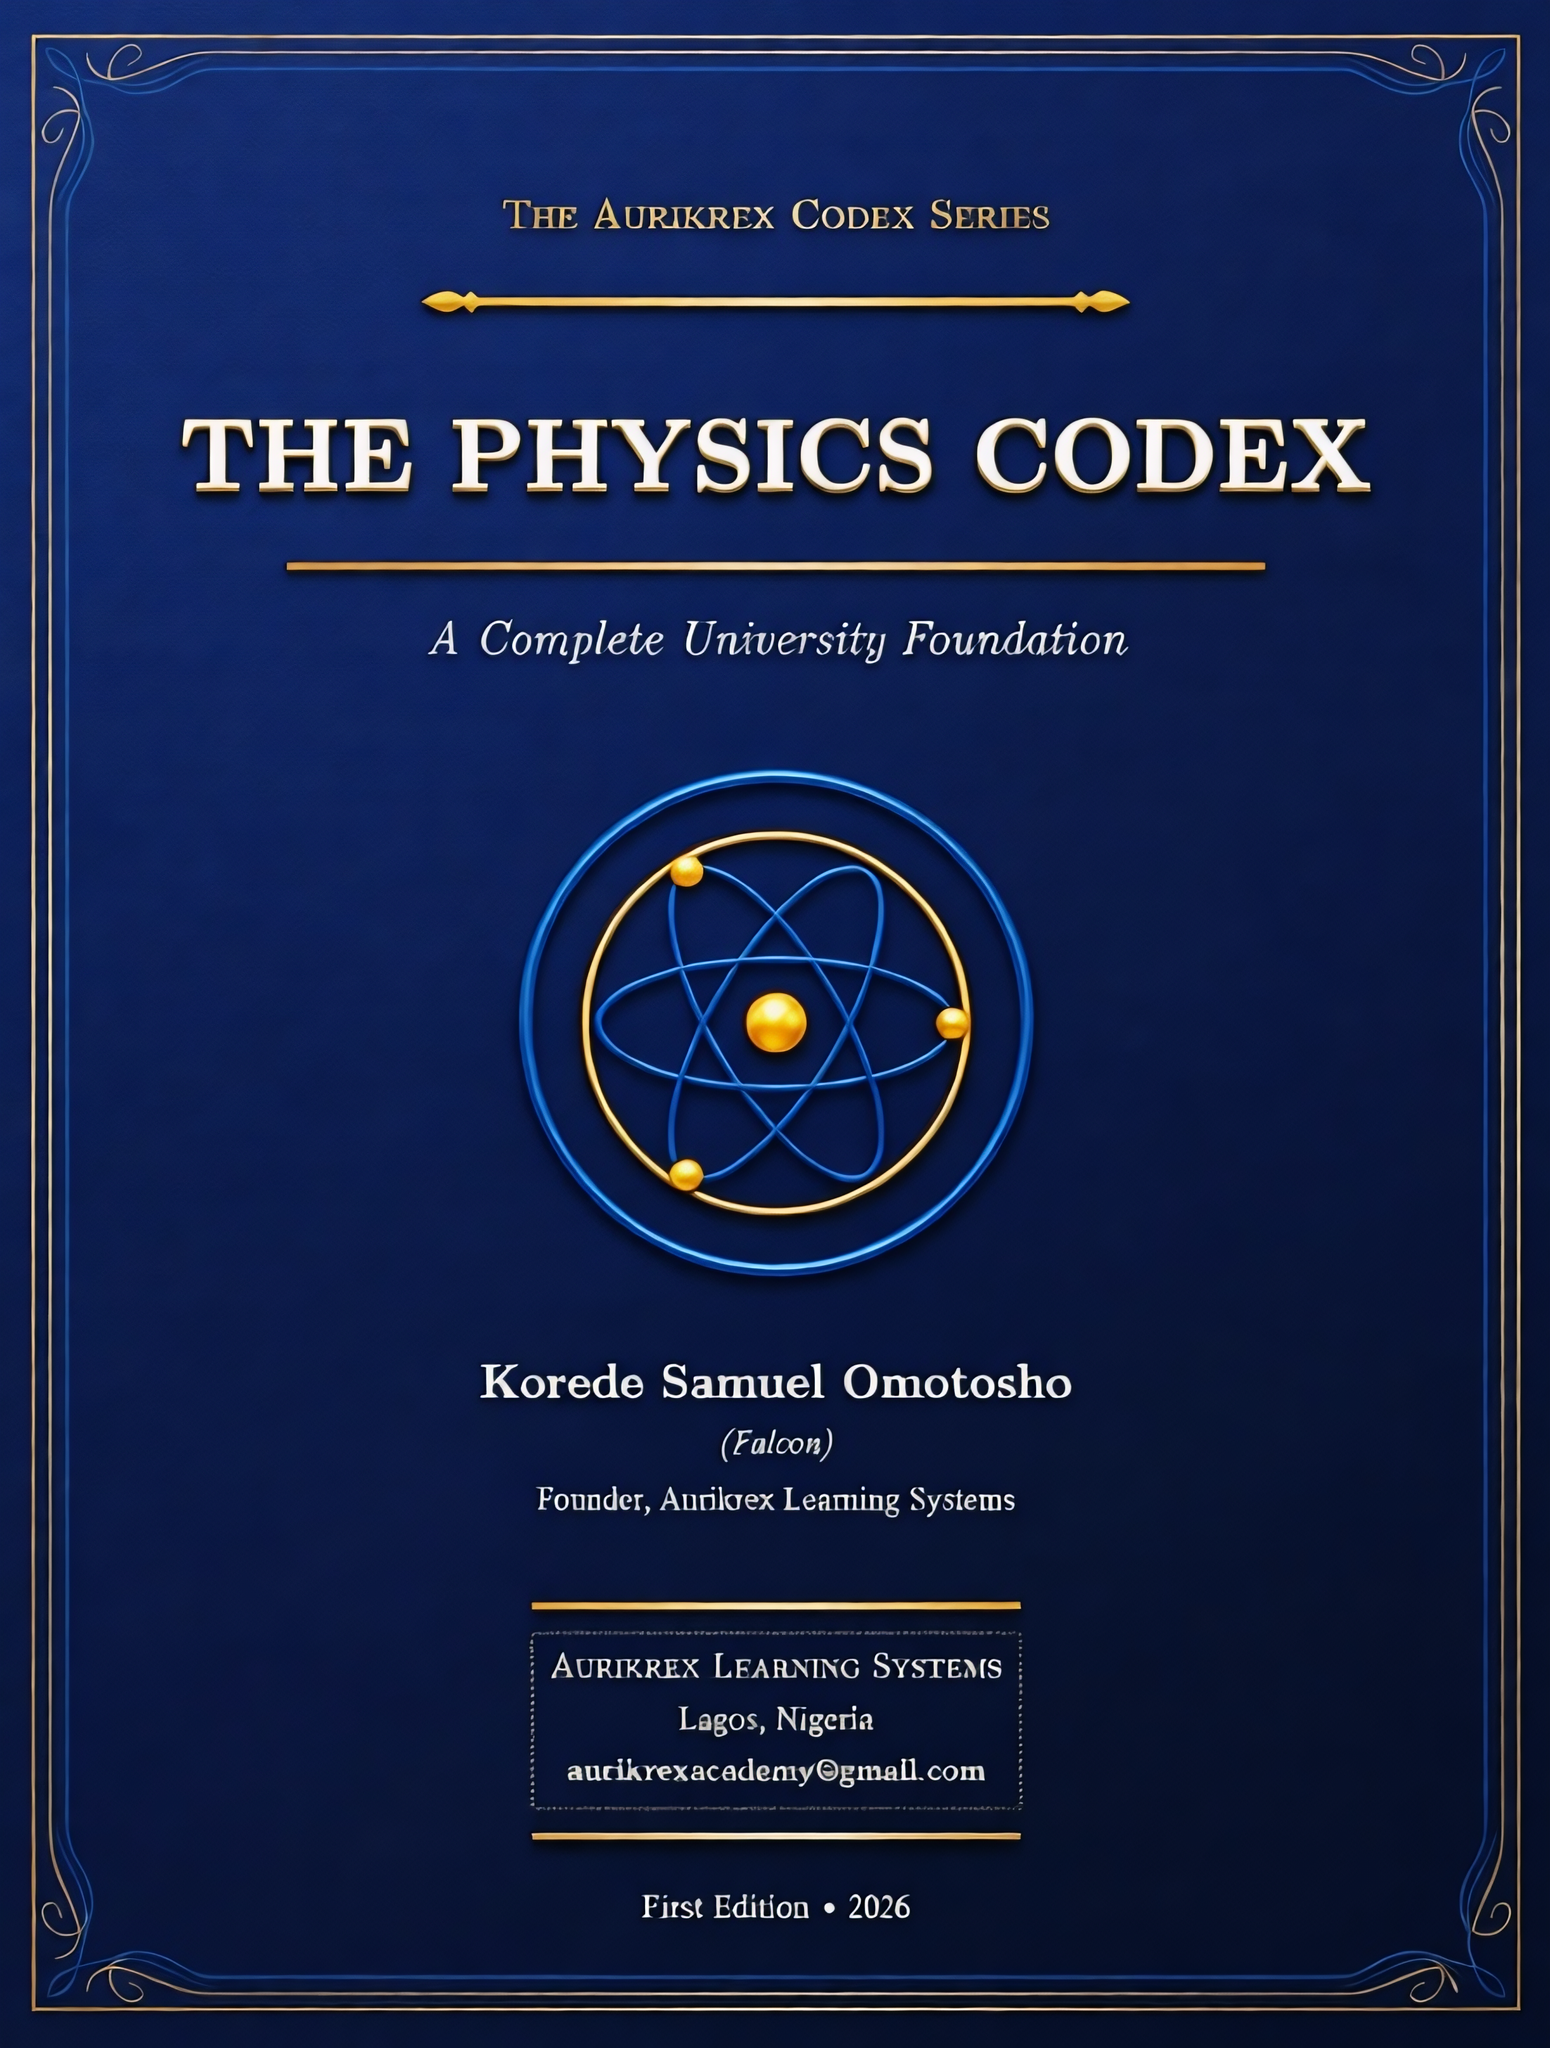
\includegraphics[width=\paperwidth,height=\paperheight]{front_cover.png}}%
}
\null\clearpage
\ClearShipoutPictureBG

% -------------------- Front matter --------------------
% Prevent \frontmatter's \cleardoublepage from inserting a blank verso page
% after the cover (common in the book class).
\let\origcleardoublepage\cleardoublepage
\let\cleardoublepage\clearpage
\frontmatter
% Keep this override active for all front-matter chapters and lists. The
% book class defaults to openright, so restoring \cleardoublepage here would
% insert blank verso pages before every \chapter* (Foreword, Preface, etc.).
\inputifexists{front_matter/titlepage}
\inputifexists{front_matter/copyright}
\inputifexists{front_matter/dedication}
\inputifexists{front_matter/foreword}
\inputifexists{front_matter/preface}
\inputifexists{front_matter/how_to_use}
\inputifexists{front_matter/about_author}

\tableofcontents
\cleardoublepage
\listoffigures
\cleardoublepage
% Restore normal open-right chapter starts for the main matter.
\let\cleardoublepage\origcleardoublepage

% -------------------- Main matter --------------------
\mainmatter
\pagestyle{fancy}

\part{Mechanics}
\inputifexists{chapters/part1_mechanics/ch01_measurement}
\inputifexists{chapters/part1_mechanics/ch02_scalars_vectors}
\inputifexists{chapters/part1_mechanics/ch03_kinematics}
\inputifexists{chapters/part1_mechanics/ch04_newtons_laws_dynamics}
\inputifexists{chapters/part1_mechanics/ch05_work_energy_power}
\inputifexists{chapters/part1_mechanics/ch06_circular_motion}
\inputifexists{chapters/part1_mechanics/ch07_simple_harmonic_motion}
\inputifexists{chapters/part1_mechanics/ch08_gravitation}
\inputifexists{chapters/part1_mechanics/ch09_elasticity}
\inputifexists{chapters/part1_mechanics/ch10_simple_machines}

\part{Fluids and Thermal Physics}
\inputifexists{chapters/part2_fluids_thermal/ch11_density_pressure_archimedes}
\inputifexists{chapters/part2_fluids_thermal/ch12_surface_tension_viscosity_capillarity}
\inputifexists{chapters/part2_fluids_thermal/ch13_temperature_thermal_expansion}
\inputifexists{chapters/part2_fluids_thermal/ch14_gas_laws_kinetic_theory}
\inputifexists{chapters/part2_fluids_thermal/ch15_heat_energy_calorimetry}
\inputifexists{chapters/part2_fluids_thermal/ch16_heat_transfer}

\part{Waves and Optics}
\inputifexists{chapters/part3_waves_optics/ch17_wave_motion}
\inputifexists{chapters/part3_waves_optics/ch18_sound_waves}
\inputifexists{chapters/part3_waves_optics/ch19_light_reflection}
\inputifexists{chapters/part3_waves_optics/ch20_light_refraction_optical_instruments}

\part{Electricity and Magnetism}
\inputifexists{chapters/part4_electricity_magnetism/ch21_electrostatics}
\inputifexists{chapters/part4_electricity_magnetism/ch22_capacitance}
\inputifexists{chapters/part4_electricity_magnetism/ch23_current_electricity}
\inputifexists{chapters/part4_electricity_magnetism/ch24_electrical_energy_power}
\inputifexists{chapters/part4_electricity_magnetism/ch25_magnetism_electromagnetism}
\inputifexists{chapters/part4_electricity_magnetism/ch26_electromagnetic_induction}

\part{Modern Physics}
\inputifexists{chapters/part5_modern_physics/ch27_atomic_structure_spectra}
\inputifexists{chapters/part5_modern_physics/ch28_radioactivity_nuclear_physics}
\inputifexists{chapters/part5_modern_physics/ch29_electronics}

% -------------------- Back matter --------------------
\backmatter
\inputifexists{back_matter/bibliography}
\appendix
\inputifexists{back_matter/appendix_a_constants}
\inputifexists{back_matter/answers}

% -------------------- Back cover (full-bleed final page) --------------------
\clearpage
\thispagestyle{empty}
\AddToShipoutPictureBG*{%
  \AtPageLowerLeft{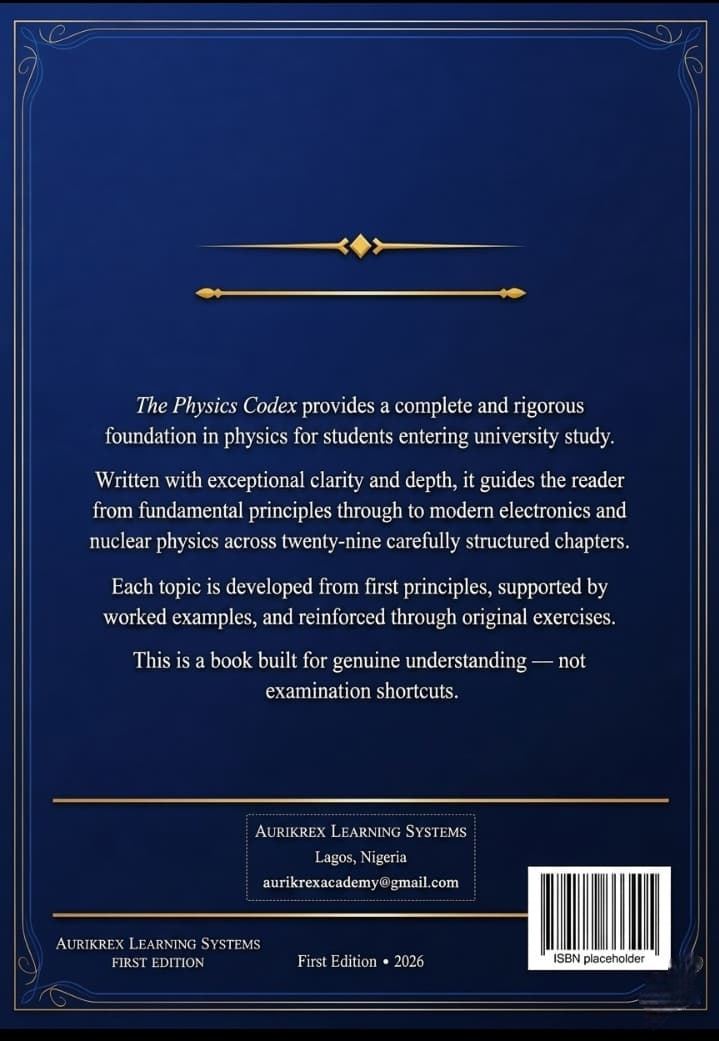
\includegraphics[width=\paperwidth,height=\paperheight]{back_cover.png}}%
}
\null\clearpage
\ClearShipoutPictureBG

\end{document}

% (Archive note: there is extra pasted content below, after \end{document}.
% It is ignored by TeX. Consider moving it into its own file if you want to keep it.)
% ============================================================
%  CHAPTER 20: REFRACTION AND OPTICAL INSTRUMENTS
%  The Physics Codex: A Complete University Foundation
%  Korede Samuel Omotosho (Falcon)
%  Aurikrex Learning Systems, 2026
%
%  File: chapters/part3/ch20_refraction_optics.tex
% ============================================================

\chapter{Refraction and Optical Instruments}
\label{ch:refraction_optics}
\minitoc
\newpage

\chapterquote{The eye is the jewel of the body.}{Henry David Thoreau}

\begin{objectivebox}
By the end of this chapter, you should be able to:
\begin{enumerate}[noitemsep]
  \item Define refraction and explain it using the
  change in wave speed at a boundary
  \item State and apply Snell's Law
  \item Define refractive index and relate it to
  wave speed
  \item Explain and calculate total internal
  reflection and critical angle
  \item Apply the lens formula and magnification
  equation to converging and diverging lenses
  \item Draw ray diagrams for lenses at various
  object positions
  \item Describe the construction and operation of
  the simple microscope, compound microscope,
  and telescope
  \item Describe defects of vision and their
  correction using lenses
  \item Define power of a lens and perform related
  calculations
\end{enumerate}
\end{objectivebox}

% ============================================================
\section{Intuition: Why Does a Straw Appear Bent?}
% ============================================================

Place a straight straw in a glass of water and look
at it from the side. The straw appears to bend at the
water surface --- the part in water seems displaced
from the part in air. Yet the straw is perfectly
straight. Nothing has bent. What has changed is the
\textit{direction of the light rays} travelling from
the straw to your eye.

Light travels at different speeds in different media.
In a vacuum it travels at $c = 3\times10^8\ \text{m\,s}^{-1}$.
In water it travels at about $2.25\times10^8\ \text{m\,s}^{-1}$.
In glass it travels at about $2\times10^8\ \text{m\,s}^{-1}$.

When light crosses a boundary from one medium to
another at an angle, the change in speed causes a
change in direction. This bending of light at a
boundary between two media is called
\textbf{refraction}, and it is the foundation of
all optical instruments --- lenses, microscopes,
telescopes, cameras, the human eye.

% ============================================================
\section{Refraction and Snell's Law}
% ============================================================

\begin{definitionbox}[Refraction]
\textbf{Refraction} is the change in direction of a
wave when it passes from one medium into another in
which it travels at a different speed. It occurs at
the boundary between the two media.

When light passes from a less dense medium (lower
refractive index, higher speed) into a denser medium
(higher refractive index, lower speed):
\begin{itemize}[noitemsep]
  \item The ray bends \textbf{toward} the normal
  \item The angle of refraction $\theta_r < \theta_i$
  \item The wavelength decreases; frequency unchanged
\end{itemize}

When light passes from a denser into a less dense medium:
\begin{itemize}[noitemsep]
  \item The ray bends \textbf{away from} the normal
  \item The angle of refraction $\theta_r > \theta_i$
\end{itemize}
\end{definitionbox}

\begin{diagbox}[Refraction at a Glass-Air Boundary]
\begin{center}
\begin{tikzpicture}[scale=1.1, font=\small]

  % Air region
  \fill[cyan!5] (0,0) rectangle (9,4.5);
  \node[gray, font=\itshape] at (1.5,4.0) {Air ($n_1 = 1.0$)};

  % Glass region
  \fill[codexblue!12] (0,-3.0) rectangle (9,0);
  \node[gray, font=\itshape] at (1.5,-2.5)
    {Glass ($n_2 = 1.5$)};

  % Interface
  \draw[very thick] (0,0) -- (9,0);
  \node[right, gray, font=\tiny] at (9,0)
    {Interface};

  % Normal
  \draw[dashed, gray, thick] (4.5,-3.2) -- (4.5,4.7);
  \node[right, gray, font=\tiny] at (4.6,4.5) {Normal};

  % Incident ray (from air into glass)
  \draw[->, very thick, codexblue, line width=2pt]
    (1.5,3.8) -- (4.5,0);
  \node[left, codexblue] at (1.3,3.6) {Incident ray};

  % Refracted ray (bends toward normal in glass)
  \draw[->, very thick, codexred, line width=2pt]
    (4.5,0) -- (6.5,-2.8);
  \node[right, codexred] at (6.6,-2.7) {Refracted ray};

  % Angle of incidence
  \draw[codexblue, thick]
    (4.5,1.0) arc(90:143:1.0);
  \node[codexblue] at (3.6,1.2) {$\theta_1$};

  % Angle of refraction (smaller, in glass)
  \draw[codexred, thick]
    (4.5,-1.0) arc(270:247:1.0);
  \node[codexred] at (4.0,-1.3) {$\theta_2$};

  % Annotations
  \node[codexblue, font=\small] at (7,3.5)
    {$\theta_1$ large (in air)};
  \node[codexred, font=\small] at (7,2.5)
    {$\theta_2$ small (in glass)};
  \node[codexgold, font=\small, align=center]
    at (7,1.5)
    {Ray bends\\toward normal\\when entering\\denser medium};

  % Partial reflection (faint)
  \draw[->, thick, codexblue!40, dashed]
    (4.5,0) -- (7.5,3.5);
  \node[right, codexblue!50, font=\tiny]
    at (7.6,3.4) {partial\\reflection};

  % Snell's Law
  \node[codexblue, font=\normalsize,
    align=center] at (2.0,1.0)
    {$n_1\sin\theta_1 = n_2\sin\theta_2$\\
    (Snell's Law)};

\end{tikzpicture}
\end{center}
\end{diagbox}

\begin{lawbox}[Snell's Law]
When light passes from medium 1 (refractive index
$n_1$) into medium 2 (refractive index $n_2$):
\[
  n_1\sin\theta_1 = n_2\sin\theta_2
\]
where $\theta_1$ is the angle of incidence and
$\theta_2$ is the angle of refraction, both measured
from the normal.
\end{lawbox}

\begin{definitionbox}[Refractive Index]
The \textbf{absolute refractive index} $n$ of a medium
is the ratio of the speed of light in vacuum to the
speed of light in the medium:
\[
  n = \frac{c}{v}
\]
where $c = 3\times10^8\ \text{m\,s}^{-1}$ is the
speed of light in vacuum and $v$ is the speed in
the medium. Since $v \leq c$, always $n \geq 1$.

The \textbf{relative refractive index} from medium
1 to medium 2:
\[
  {}_1n_2 = \frac{n_2}{n_1} = \frac{v_1}{v_2}
  = \frac{\sin\theta_1}{\sin\theta_2}
\]
\end{definitionbox}

\begin{table}[H]
\centering
\caption{Refractive Indices of Common Materials}
\label{tab:refractive_index}
\begin{tabular}{ll}
\toprule
\textbf{Medium} & \textbf{Refractive Index $n$}\\
\midrule
Vacuum & 1.000 (exactly)\\
Air & 1.0003 $\approx$ 1.00\\
Water (20°C) & 1.333\\
Crown glass & 1.50\\
Dense glass & 1.60--1.70\\
Diamond & 2.42\\
Ice & 1.31\\
Ethanol & 1.36\\
\bottomrule
\end{tabular}
\end{table}

\begin{examplebox}[20.1]
\stepcounter{workedexample}
A ray of light in air strikes a glass surface
($n = 1.50$) at an angle of incidence of $40°$.\\
(a) Find the angle of refraction.\\
(b) Find the speed of light in the glass.\\
(c) Find the wavelength in glass if the wavelength
in air is $600\ \text{nm}$.
\end{examplebox}

\begin{solutionbox}
\textbf{(a)} Snell's Law ($n_{air} = 1.00$):
\[
  \sin\theta_2 = \frac{n_1\sin\theta_1}{n_2}
  = \frac{1.00 \times \sin 40°}{1.50}
  = \frac{0.6428}{1.50} = 0.4285
\]
\[
  \theta_2 = \sin^{-1}(0.4285) = 25.4°
\]
The ray bends toward the normal on entering the
denser glass ($25.4° < 40°$).

\textbf{(b)} Speed in glass:
\[
  v = \frac{c}{n} = \frac{3.0\times10^8}{1.50}
  = 2.0\times10^8\ \text{m\,s}^{-1}
\]

\textbf{(c)} Wavelength in glass. Frequency is
unchanged at a boundary; only speed and wavelength change:
\[
  \lambda_{glass} = \frac{\lambda_{air}}{n}
  = \frac{600\ \text{nm}}{1.50} = 400\ \text{nm}
\]
The light has the same colour (frequency) but shorter
wavelength in glass. This is why a spectrum appears
when white light passes through a prism --- different
colours (frequencies) refract by different amounts
(dispersion).
\end{solutionbox}

% ============================================================
\section{Total Internal Reflection}
% ============================================================

When light travels from a denser medium into a less
dense medium, the refracted ray bends away from the
normal. As the angle of incidence increases, the
angle of refraction also increases. At a certain
critical angle $\theta_c$, the refracted ray runs
along the surface ($\theta_r = 90°$). Beyond this
angle, refraction is impossible --- all the light is
reflected back into the denser medium. This is
\textbf{total internal reflection}.

\begin{definitionbox}[Critical Angle and Total Internal
Reflection]
\textbf{Total internal reflection} (TIR) occurs when:
\begin{enumerate}[noitemsep]
  \item Light travels from a \textit{denser} to a
  \textit{less dense} medium (from higher $n$ to
  lower $n$)
  \item The angle of incidence exceeds the
  \textbf{critical angle} $\theta_c$
\end{enumerate}

At the critical angle, $\theta_r = 90°$:
\[
  n_1\sin\theta_c = n_2\sin 90° = n_2
\]
\[
  \boxed{\sin\theta_c = \frac{n_2}{n_1}}
\]
For glass to air ($n_2 = 1$):
$\sin\theta_c = 1/n_1$, so $\theta_c
= \sin^{-1}(1/n_1)$.
\end{definitionbox}

\begin{diagbox}[Total Internal Reflection: Three Cases]
\begin{center}
\begin{tikzpicture}[scale=0.95, font=\small]

  % Glass (bottom, denser)
  \fill[codexblue!12] (0,-2.8) rectangle (13,0);
  \draw[very thick] (0,0) -- (13,0);
  % Air (top)
  \fill[cyan!5] (0,0) rectangle (13,3.0);

  % Labels
  \node[gray, font=\itshape] at (1.0,2.5)
    {Air ($n_2$)};
  \node[gray, font=\itshape] at (1.0,-2.3)
    {Glass ($n_1 > n_2$)};

  % === Case 1: Below critical angle ===
  \begin{scope}[shift={(1.5,0)}]
    % Normal
    \draw[dashed, gray] (0,-3.0) -- (0,3.0);
    % Incident
    \draw[->, thick, codexblue]
      (-1.5,-2.5) -- (0,0);
    % Refracted (bends away)
    \draw[->, thick, codexred]
      (0,0) -- (1.5,2.5);
    % Weak reflected
    \draw[->, thin, codexblue!40, dashed]
      (0,0) -- (1.5,-2.5);
    \node[font=\tiny, align=center] at (0,-3.2)
      {$\theta_i < \theta_c$\\mostly refracted};
    \draw[codexblue, thin]
      (0,-0.8) arc(270:241:0.8);
    \node[codexblue, font=\tiny] at (-0.4,-1.1)
      {$\theta_i$};
    \draw[codexred, thin]
      (0,0.8) arc(90:60:0.8);
    \node[codexred, font=\tiny] at (0.5,1.0)
      {$\theta_r$};
  \end{scope}

  % === Case 2: At critical angle ===
  \begin{scope}[shift={(5.5,0)}]
    % Normal
    \draw[dashed, gray] (0,-3.0) -- (0,3.0);
    % Incident
    \draw[->, thick, codexblue]
      (-2.0,-2.0) -- (0,0);
    % Refracted along surface
    \draw[->, thick, codexred]
      (0,0) -- (3.0,0);
    \node[codexred, font=\tiny, right] at (3.1,0.1)
      {refracted ray\\along surface};
    % Reflected
    \draw[->, thin, codexblue!60, dashed]
      (0,0) -- (2.0,-2.0);
    \node[font=\tiny, align=center] at (0,-3.2)
      {$\theta_i = \theta_c$\\$\theta_r = 90°$};
    \draw[codexblue, thin]
      (0,-0.7) arc(270:225:0.7);
    \node[codexblue, font=\tiny] at (-0.4,-1.0)
      {$\theta_c$};
  \end{scope}

  % === Case 3: Above critical angle (TIR) ===
  \begin{scope}[shift={(10.5,0)}]
    % Normal
    \draw[dashed, gray] (0,-3.0) -- (0,3.0);
    % Incident
    \draw[->, thick, codexblue]
      (-2.2,-1.8) -- (0,0);
    % NO refracted ray
    \draw[codexred!30, very thick, dashed]
      (0,0) -- (2.0,0.5);
    \node[codexred!40, font=\tiny] at (2.5,0.7)
      {no refraction};
    % Total internal reflection
    \draw[->, very thick, codexred, line width=2pt]
      (0,0) -- (2.2,-1.8);
    \node[codexred, font=\small] at (1.0,-2.5)
      {TIR};
    \node[font=\tiny, align=center] at (0,-3.2)
      {$\theta_i > \theta_c$\\Total Internal\\Reflection};
    \draw[codexblue, thin]
      (0,-0.7) arc(270:219:0.7);
    \draw[codexred, thin]
      (0,-0.7) arc(270:321:0.7);
  \end{scope}

\end{tikzpicture}
\end{center}
\end{diagbox}

\begin{examplebox}[20.2]
\stepcounter{workedexample}
Light travels from glass ($n = 1.52$) into water
($n = 1.33$).\\
(a) Calculate the critical angle.\\
(b) Calculate the critical angle for glass-air.\\
(c) A fibre optic cable uses glass of $n = 1.55$
with a cladding of $n = 1.45$. Find the critical
angle and state why TIR is useful in optical fibres.
\end{examplebox}

\begin{solutionbox}
\textbf{(a)} Glass to water:
\[
  \sin\theta_c = \frac{n_{water}}{n_{glass}}
  = \frac{1.33}{1.52} = 0.875
\]
\[
  \theta_c = \sin^{-1}(0.875) = 61.0°
\]

\textbf{(b)} Glass to air ($n_{air} = 1.00$):
\[
  \sin\theta_c = \frac{1.00}{1.52} = 0.658
  \implies \theta_c = 41.1°
\]

\textbf{(c)} Core-cladding:
\[
  \sin\theta_c = \frac{1.45}{1.55} = 0.9355
  \implies \theta_c = 69.4°
\]

Any ray hitting the core-cladding boundary at more
than $69.4°$ from the normal (i.e.\ nearly parallel
to the fibre axis) undergoes TIR and is trapped
inside the fibre. Since the glass bends, the angles
adjust to stay above the critical angle throughout
the bend. Light can travel thousands of kilometres
through optical fibres with very little loss ---
the entire modern internet depends on this.
\end{solutionbox}

\begin{realworldbox}[Optical Fibres and the Internet]
The fibre optic cables that carry the internet
across oceans use total internal reflection. Light
pulses, each encoding billions of bits per second,
are trapped inside glass fibres (diameter $\sim 10\
\mu\text{m}$) by TIR and travel thousands of
kilometres from continent to continent. A single
hair-thin glass fibre can carry more data than a
copper cable the thickness of an arm. The submarine
cable landing stations along the West African
coast --- in Lagos, Accra, Dakar --- are where
these fibre cables connect Africa to the rest of
the global internet.
\end{realworldbox}

% ============================================================
\section{Thin Lenses}
% ============================================================

\begin{definitionbox}[Converging and Diverging Lenses]
A \textbf{converging (convex) lens} is thicker at
the centre than at the edges. It refracts parallel
rays to converge at the focal point F on the
far side. Focal length $f > 0$.

A \textbf{diverging (concave) lens} is thinner at
the centre. It refracts parallel rays to diverge,
appearing to come from the focal point F on the
same side as the incoming light. Focal length $f < 0$.
\end{definitionbox}

\begin{diagbox}[Converging and Diverging Lenses]
\begin{center}
\begin{tikzpicture}[scale=0.95, font=\small]

  % === CONVERGING LENS ===
  \begin{scope}[shift={(0,0)}]
    \node[font=\bfseries, codexblue] at (4.5,4.2)
      {Converging (Convex) Lens};

    % Lens shape
    \fill[codexblue!15]
      (4,0) .. controls (3.5,1.5) and (3.5,3) ..
      (4,4.0) .. controls (4.5,3) and (4.5,1.5) ..
      (4,0);
    \draw[very thick, codexblue]
      (4,0) .. controls (3.5,1.5) and (3.5,3) ..
      (4,4.0) .. controls (4.5,3) and (4.5,1.5) ..
      (4,0);

    % Principal axis
    \draw[dashed, gray] (0,2.0) -- (8.5,2.0);

    % Focal points
    \fill[codexgold] (2.0,2.0) circle (4pt)
      node[below]{\small F};
    \fill[codexgold] (6.0,2.0) circle (4pt)
      node[below]{\small F$'$};
    \draw[<->, gray] (4.0,1.0) -- (6.0,1.0);
    \node[below, gray, font=\tiny] at (5.0,0.9)
      {$f$};

    % Three parallel rays converging to F'
    \foreach \h/\col in {
      0.5/codexblue!60,
      2.0/codexblue,
      3.5/codexblue!60} {
      \draw[->, thick, \col]
        (0.5,\h) -- (4.0,\h);
    }
    % Refracted rays converge to F'
    \draw[->, thick, codexblue!60]
      (4.0,0.5) -- (6.0,2.0);
    \draw[->, thick, codexblue]
      (4.0,2.0) -- (6.0,2.0);
    \draw[->, thick, codexblue!60]
      (4.0,3.5) -- (6.0,2.0);

    % Lines from F' onwards
    \draw[codexblue!40, dashed]
      (6.0,2.0) -- (8.0,2.0);
  \end{scope}

  % === DIVERGING LENS ===
  \begin{scope}[shift={(10,0)}]
    \node[font=\bfseries, codexred] at (3.5,4.2)
      {Diverging (Concave) Lens};

    % Lens shape (concave = thinner at centre)
    \fill[codexred!15]
      (3.5,0) .. controls (4.0,1.5) and (4.0,2.5)
      .. (3.5,4.0) -- (4.5,4.0) ..
      controls (4.0,2.5) and (4.0,1.5) ..
      (4.5,0) -- cycle;
    \draw[very thick, codexred]
      (3.5,0) .. controls (4.0,1.5) and (4.0,2.5)
      .. (3.5,4.0);
    \draw[very thick, codexred]
      (4.5,0) .. controls (4.0,1.5) and (4.0,2.5)
      .. (4.5,4.0);

    % Principal axis
    \draw[dashed, gray] (-1,2.0) -- (8.5,2.0);

    % Virtual focal point (same side as incoming)
    \fill[codexgold!70] (2.0,2.0) circle (4pt)
      node[below]{\small F (virtual)};
    \draw[<->, gray] (2.0,1.0) -- (4.0,1.0);
    \node[below, gray, font=\tiny] at (3.0,0.9)
      {$|f|$};

    % Parallel rays diverging
    \foreach \h/\col in {
      0.5/codexred!60,
      2.0/codexred,
      3.5/codexred!60} {
      \draw[->, thick, \col]
        (-0.5,\h) -- (3.9,\h);
    }
    % Diverged rays
    \draw[->, thick, codexred!60]
      (4.1,0.5) -- (6.5,0.0);
    \draw[->, thick, codexred]
      (4.1,2.0) -- (6.5,2.0);
    \draw[->, thick, codexred!60]
      (4.1,3.5) -- (6.5,4.0);
    % Dashed extensions back to virtual F
    \draw[dashed, codexred!50]
      (4.1,0.5) -- (2.0,2.0);
    \draw[dashed, codexred!50]
      (4.1,3.5) -- (2.0,2.0);

  \end{scope}

\end{tikzpicture}
\end{center}
\end{diagbox}

% ============================================================
\section{The Lens Formula and Magnification}
% ============================================================

\begin{lawbox}[The Lens Formula]
For a thin lens with focal length $f$, object
distance $u$, and image distance $v$:
\[
  \frac{1}{f} = \frac{1}{v} - \frac{1}{u}
\]
or equivalently:
\[
  \frac{1}{f} = \frac{1}{v} + \frac{1}{u}
  \quad \text{(using the real-is-positive convention)}
\]

\textbf{Sign convention (Real-is-Positive):}
\begin{itemize}[noitemsep]
  \item $u$ is always positive for real objects
  \item Converging lens: $f > 0$
  \item Diverging lens: $f < 0$
  \item Real images: $v > 0$ (image on opposite
  side of lens from object)
  \item Virtual images: $v < 0$ (image on same
  side as object)
\end{itemize}
\end{lawbox}

\begin{lawbox}[Power of a Lens]
The \textbf{power} $P$ of a lens is the reciprocal
of its focal length in metres:
\[
  P = \frac{1}{f(\text{in metres})}
\]
SI unit: dioptre (D) where $1\ \text{D}
= 1\ \text{m}^{-1}$.

Converging lens: $P > 0$.
Diverging lens: $P < 0$.

For lenses in contact:
$P_{total} = P_1 + P_2$
\end{lawbox}

\begin{examplebox}[20.3]
\stepcounter{workedexample}
An object $5.0\ \text{cm}$ tall is placed
$25\ \text{cm}$ from a converging lens of focal
length $10\ \text{cm}$.\\
(a) Find the image distance.\\
(b) Find the magnification and image height.\\
(c) Describe the image.
\end{examplebox}

\begin{solutionbox}
$u = 25\ \text{cm}$, $f = +10\ \text{cm}$

\textbf{(a)} Using $\frac{1}{v} = \frac{1}{f}
- \frac{1}{u}$:

Wait --- using the standard form for lenses:
$\frac{1}{f} = \frac{1}{v} - \frac{1}{u}$ with
the new Cartesian convention
($u$ negative for real object),
or more practically using:
\[
  \frac{1}{v} = \frac{1}{f} + \frac{1}{u}
  \quad\text{(real-is-positive, }u\text{ positive)}
\]

Actually, to be consistent with UTME and Nigerian
textbook convention:
\[
  \frac{1}{v} = \frac{1}{f} - \frac{1}{u}
  = \frac{1}{10} - \frac{1}{25}
  = \frac{5-2}{50} = \frac{3}{50}
\]
\[
  v = \frac{50}{3} = 16.7\ \text{cm}
\]

\textbf{(b)} Magnification:
\[
  m = \frac{v}{u} = \frac{16.7}{25} = +0.67
\]
Image height $= 0.67 \times 5.0 = 3.3\ \text{cm}$

\textbf{(c)} The image is: real (positive $v$,
on opposite side), erect in this convention
(positive $m$), diminished ($|m| < 1$),
at $16.7\ \text{cm}$ beyond the lens.
\end{solutionbox}

\begin{examtipbox}
Nigerian UTME uses the \textbf{real-is-positive}
convention where both $u$ and $v$ are positive for
real objects and images. The lens formula then reads:
$\frac{1}{f} = \frac{1}{v} - \frac{1}{u}$ with the
magnification $m = v/u$. For a diverging lens, $f$
is negative. For a virtual image, $v$ is negative.
Always state your sign convention clearly.
\end{examtipbox}

\begin{table}[H]
\centering
\caption{Images Formed by a Converging Lens}
\label{tab:lens_images}
\small
\begin{tabular}{p{3cm}p{2.5cm}p{2cm}p{2cm}p{2cm}}
\toprule
\textbf{Object position} & \textbf{Image position} &
\textbf{Size} & \textbf{Nature} &
\textbf{Orientation}\\
\midrule
At infinity & At F & Point & Real & Inverted\\
Beyond $2f$ & Between F and $2f$ & Smaller &
  Real & Inverted\\
At $2f$ & At $2f$ & Same & Real & Inverted\\
Between F and $2f$ & Beyond $2f$ & Larger &
  Real & Inverted\\
At F & At infinity & --- & --- & ---\\
Inside F & Same side & Larger & Virtual & Erect\\
\bottomrule
\end{tabular}
\end{table}

% ============================================================
\section{The Simple Microscope (Magnifying Glass)}
% ============================================================

\begin{processbox}[The Simple Microscope]
A simple microscope is just a single converging
lens used to view a small object placed within
the focal length. The object distance $u < f$,
producing a virtual, erect, magnified image.

For normal adjustment (image at infinity,
least strain for the eye):
\[
  M = \frac{D}{f}
\]
where $D = 25\ \text{cm}$ is the near point
(least distance of distinct vision) and $f$ is
the focal length of the lens.

For adjustment at near point $D$:
\[
  M = 1 + \frac{D}{f}
\]
\end{processbox}

\begin{examplebox}[20.4]
\stepcounter{workedexample}
A magnifying glass has a focal length of $5.0\ \text{cm}$.
Taking $D = 25\ \text{cm}$:\\
(a) Find the magnifying power for normal adjustment.\\
(b) Find the magnifying power when the image is at
the near point.\\
(c) At what position must the object be placed for
the image to be at infinity?
\end{examplebox}

\begin{solutionbox}
\textbf{(a)} Normal adjustment:
\[
  M = \frac{D}{f} = \frac{25}{5.0} = 5\times
\]

\textbf{(b)} Image at near point:
\[
  M = 1 + \frac{D}{f} = 1 + \frac{25}{5.0} = 6\times
\]

\textbf{(c)} For image at infinity, the object must
be at the focal point: $u = f = 5.0\ \text{cm}$ from
the lens.
\end{solutionbox}

% ============================================================
\section{The Compound Microscope}
% ============================================================

\begin{processbox}[The Compound Microscope]
A compound microscope uses two converging lenses
to achieve high magnification:
\begin{itemize}[noitemsep]
  \item \textbf{Objective lens} (short focal length
  $f_o$): object is placed just beyond $f_o$,
  forming a real, inverted, magnified image
  (\textit{primary image}) inside the tube.
  \item \textbf{Eyepiece lens} (short focal length
  $f_e$): acts as a magnifying glass to view the
  primary image, forming a final virtual, magnified
  image for the eye.
\end{itemize}
Total magnification (approximately):
\[
  M_{total} = m_o \times M_e
  = \frac{v_o}{u_o} \times \frac{D}{f_e}
\]
where $v_o$ is the image distance of the objective
and $u_o$ is the object distance for the objective.
For normal adjustment (final image at infinity):
\[
  M_{total} = \frac{L}{f_o} \times \frac{D}{f_e}
\]
where $L$ is the length of the tube.
\end{processbox}

\begin{diagbox}[The Compound Microscope: Ray Diagram]
\begin{center}
\begin{tikzpicture}[scale=0.8, font=\small]

  % Objective lens
  \fill[codexblue!20]
    (2.0,2.5) .. controls (1.7,3.5) and (1.7,5.5)
    .. (2.0,6.5) .. controls (2.3,5.5) and (2.3,3.5)
    .. (2.0,2.5);
  \draw[very thick, codexblue]
    (2.0,2.5) .. controls (1.7,3.5) and (1.7,5.5)
    .. (2.0,6.5) .. controls (2.3,5.5) and (2.3,3.5)
    .. (2.0,2.5);
  \node[below, codexblue] at (2.0,2.3)
    {Objective\\$f_o$ (small)};

  % Eyepiece lens
  \fill[codexred!20]
    (9.0,2.0) .. controls (8.6,4.5) and (8.6,7.5)
    .. (9.0,10.0) .. controls (9.4,7.5) and (9.4,4.5)
    .. (9.0,2.0);
  \draw[very thick, codexred]
    (9.0,2.0) .. controls (8.6,4.5) and (8.6,7.5)
    .. (9.0,10.0) .. controls (9.4,7.5) and (9.4,4.5)
    .. (9.0,2.0);
  \node[below, codexred] at (9.0,1.8)
    {Eyepiece\\$f_e$ (small)};

  % Principal axis
  \draw[dashed, gray] (0,4.5) -- (13,4.5);

  % Object (small, just beyond F_o)
  \draw[->, very thick, codexblue, line width=2pt]
    (0.8,4.5) -- (0.8,5.8);
  \node[left, codexblue, font=\tiny] at (0.7,5.1)
    {Object};

  % F_o
  \fill[codexgold] (1.5,4.5) circle (3pt)
    node[below, font=\tiny]{$F_o$};

  % Primary image (real, inverted, magnified)
  \draw[->, very thick, codexgold, line width=2pt]
    (7.0,4.5) -- (7.0,2.5);
  \node[right, codexgold, font=\tiny] at (7.1,3.5)
    {Primary image\\(real, inverted)};

  % F_e (primary image inside F_e of eyepiece)
  \fill[codexred!60] (8.2,4.5) circle (3pt)
    node[below, font=\tiny]{$F_e$};

  % Rays from object through objective
  \draw[->, thick, codexblue]
    (0.8,5.8) -- (2.0,5.8);
  \draw[thick, codexblue] (2.0,5.8) -- (7.0,2.5);

  \draw[->, thick, codexblue!60]
    (0.8,5.8) -- (1.5,4.5);
  \draw[thick, codexblue!60] (1.5,4.5) -- (2.0,4.5);
  \draw[thick, codexblue!60] (2.0,4.5) -- (7.0,2.5);

  % Rays from primary image through eyepiece
  \draw[->, thick, codexred]
    (7.0,2.5) -- (9.0,2.5);
  \draw[->, thick, codexred]
    (9.0,2.5) -- (11.0,1.0);

  \draw[->, thick, codexred!60]
    (7.0,2.5) -- (9.0,4.5);
  \draw[->, thick, codexred!60]
    (9.0,4.5) -- (11.0,4.5);

  % Final virtual image (dashed, goes off left)
  \draw[dashed, codexred!50]
    (9.0,2.5) -- (5.0,6.5);
  \draw[dashed, codexred!50]
    (9.0,4.5) -- (5.0,6.5);
  \fill[codexred!40] (5.0,6.5) circle (4pt);
  \node[above, codexred!60, font=\tiny]
    at (5.0,6.7) {Final virtual image\\(large, inverted)};

  % Eye
  \fill[gray!40] (11.5,4.5) circle (6pt);
  \node[right, gray, font=\small] at (11.7,4.5)
    {Eye};

  % Tube length
  \draw[<->, gray] (2.1,1.5) -- (8.9,1.5);
  \node[below, gray, font=\tiny] at (5.5,1.4)
    {Tube length $L$};

\end{tikzpicture}
\end{center}
\end{diagbox}

% ============================================================
\section{The Astronomical Telescope}
% ============================================================

\begin{processbox}[The Astronomical (Refracting) Telescope]
An astronomical telescope uses two converging lenses
to view distant objects:
\begin{itemize}[noitemsep]
  \item \textbf{Objective lens} (large diameter,
  long focal length $f_o$): collects light from a
  distant object, forming a real, diminished,
  inverted image at its focal plane.
  \item \textbf{Eyepiece lens} (short focal length
  $f_e$): magnifies the image formed by the objective.
\end{itemize}

For normal adjustment (final image at infinity):
\begin{itemize}[noitemsep]
  \item The focal points of objective and eyepiece
  coincide (objective image at eyepiece focal point)
  \item Tube length $= f_o + f_e$
\end{itemize}

Angular magnification:
\[
  M = \frac{f_o}{f_e}
\]
For high magnification: large $f_o$, small $f_e$.
\end{processbox}

\begin{examplebox}[20.5]
\stepcounter{workedexample}
An astronomical telescope has an objective of focal
length $100\ \text{cm}$ and an eyepiece of focal
length $5.0\ \text{cm}$.\\
(a) Find the angular magnification for normal
adjustment.\\
(b) Find the length of the telescope tube.\\
(c) If the eyepiece is replaced with one of focal
length $2.5\ \text{cm}$, what is the new magnification?
\end{examplebox}

\begin{solutionbox}
\textbf{(a)} Magnification:
\[
  M = \frac{f_o}{f_e} = \frac{100}{5.0} = 20\times
\]

\textbf{(b)} Tube length:
\[
  L = f_o + f_e = 100 + 5.0 = 105\ \text{cm}
\]

\textbf{(c)} With new eyepiece:
\[
  M = \frac{100}{2.5} = 40\times
\]
Halving the eyepiece focal length doubles the
magnification, but makes it harder to design (shorter
focal length requires smaller, harder-to-manufacture
lenses with greater aberration).
\end{solutionbox}

% ============================================================
\section{Defects of Vision and Their Correction}
% ============================================================

\begin{diagbox}[Short-sight (Myopia) and Long-sight (Hypermetropia)]
\begin{center}
\begin{tikzpicture}[scale=0.9, font=\small]

  % === SHORT-SIGHT (Myopia) ===
  \begin{scope}[shift={(0,5)}]
    \node[font=\bfseries, codexred] at (4.5,2.0)
      {Short-sight (Myopia): Image forms in front of retina};

    % Eyeball
    \fill[white] (5,0) circle (1.5cm);
    \draw[very thick] (5,0) circle (1.5cm);
    % Lens of eye
    \fill[cyan!30] (3.6,-0.3) .. controls (3.4,0)
      and (3.4,0) .. (3.6,0.3) ..
      controls (3.8,0) and (3.8,0) .. (3.6,-0.3);
    % Retina
    \draw[codexgreen, very thick]
      (5,0) ++(20:1.5) arc(20:-20:1.5);
    \node[codexgreen, font=\tiny] at (6.4,0) {Retina};
    % Focal point (in front of retina - SHORT SIGHT)
    \fill[codexred] (5.2,0) circle (4pt);
    \node[above, codexred, font=\tiny] at (5.2,0.1)
      {image here};
    % Rays converging too soon
    \draw[->, thick, codexblue]
      (0.5,0.8) -- (3.5,0.3);
    \draw[->, thick, codexblue]
      (0.5,-0.8) -- (3.5,-0.3);
    \draw[thick, codexred] (3.5,0.3) -- (5.2,0);
    \draw[thick, codexred] (3.5,-0.3) -- (5.2,0);
    % Diverge after focal point
    \draw[dashed, codexred!50]
      (5.2,0) -- (6.5,0.4);
    \draw[dashed, codexred!50]
      (5.2,0) -- (6.5,-0.4);
    \node[font=\tiny, align=center] at (2.0,-1.5)
      {Corrected by:\\diverging (concave) lens\\
      $P < 0$};
  \end{scope}

  % === LONG-SIGHT (Hypermetropia) ===
  \begin{scope}[shift={(0,0)}]
    \node[font=\bfseries, codexblue] at (4.5,2.0)
      {Long-sight (Hypermetropia): Image forms behind retina};

    % Eyeball
    \fill[white] (5,0) circle (1.5cm);
    \draw[very thick] (5,0) circle (1.5cm);
    % Lens
    \fill[cyan!30] (3.6,-0.3) .. controls (3.4,0)
      and (3.4,0) .. (3.6,0.3) ..
      controls (3.8,0) and (3.8,0) .. (3.6,-0.3);
    % Retina
    \draw[codexgreen, very thick]
      (5,0) ++(20:1.5) arc(20:-20:1.5);
    \node[codexgreen, font=\tiny] at (6.4,0) {Retina};
    % Focal point (beyond retina - LONG SIGHT)
    \fill[codexblue] (7.5,0) circle (4pt);
    \node[above, codexblue, font=\tiny] at (7.5,0.1)
      {image would form here};
    % Rays not converging enough
    \draw[->, thick, codexblue]
      (0.5,0.8) -- (3.5,0.3);
    \draw[->, thick, codexblue]
      (0.5,-0.8) -- (3.5,-0.3);
    \draw[thick, codexblue] (3.5,0.3) -- (6.4,0.2);
    \draw[thick, codexblue] (3.5,-0.3) -- (6.4,-0.2);
    \node[font=\tiny, align=center] at (2.0,-1.5)
      {Corrected by:\\converging (convex) lens\\
      $P > 0$};
  \end{scope}

\end{tikzpicture}
\end{center}
\end{diagbox}

\begin{table}[H]
\centering
\caption{Defects of Vision and Their Correction}
\label{tab:vision_defects}
\begin{tabular}{llll}
\toprule
\textbf{Defect} & \textbf{Cause} & \textbf{Effect} &
\textbf{Correction}\\
\midrule
Short-sight (myopia) &
  Eyeball too long or lens & Cannot see & Diverging
  \\
& too curved; image in & distant objects & (concave)
  lens\\
& front of retina & clearly & \\[4pt]
Long-sight &
  Eyeball too short or & Cannot see & Converging
  \\
(hypermetropia) &
  lens too flat; image & near objects & (convex) lens
  \\
& behind retina & clearly & \\[4pt]
Astigmatism &
  Uneven curvature & Blurred & Cylindrical lens
  \\
& of cornea/lens & vision & \\[4pt]
Presbyopia &
  Age-related loss & Difficulty & Converging lens
  \\
& of lens flexibility & reading & (reading glasses)\\
\bottomrule
\end{tabular}
\end{table}

\begin{examplebox}[20.6]
\stepcounter{workedexample}
A short-sighted person can see clearly up to a maximum
distance of $0.50\ \text{m}$ (far point). What lens is
needed for them to see objects at infinity clearly?
\end{examplebox}

\begin{solutionbox}
The correcting lens must produce a virtual image of
a distant object (at infinity) at the person's far
point ($0.50\ \text{m}$).

$u = \infty$ (object at infinity),
$v = -0.50\ \text{m}$ (virtual image at far point,
same side as object --- negative)

\[
  \frac{1}{f} = \frac{1}{v} - \frac{1}{u}
  = \frac{1}{-0.50} - \frac{1}{\infty}
  = -2.0 - 0 = -2.0\ \text{m}^{-1}
\]

Power: $P = -2.0\ \text{D}$ (diverging lens).

A $-2.0\ \text{D}$ diverging lens corrects this
short-sightedness.
\end{solutionbox}

% ============================================================
\section{Chapter Summary}
% ============================================================

\begin{summarybox}
\textbf{Refraction:} light bends at a boundary due
to change in speed.
Toward normal when entering denser medium.

\textbf{Snell's Law:}
$n_1\sin\theta_1 = n_2\sin\theta_2$

\textbf{Refractive index:} $n = c/v$;
$\lambda_{medium} = \lambda_{vacuum}/n$.
Frequency unchanged at boundary.

\textbf{Critical angle:}
$\sin\theta_c = n_2/n_1$ (denser to less dense).
TIR occurs when $\theta_i > \theta_c$.

\textbf{Lens formula:}
$\frac{1}{f} = \frac{1}{v} - \frac{1}{u}$
(real-is-positive convention)

Converging lens: $f > 0$.
Diverging lens: $f < 0$.
Magnification: $m = v/u$.

\textbf{Power:} $P = 1/f$ (dioptres D);
lenses in contact: $P_{total} = P_1 + P_2$.

\textbf{Simple microscope:}
$M = D/f$ (normal adjustment).

\textbf{Compound microscope:}
$M = (L/f_o)(D/f_e)$.

\textbf{Telescope:}
$M = f_o/f_e$; tube length $= f_o + f_e$.

\textbf{Short-sight:} corrected by diverging lens
($P < 0$). \textbf{Long-sight:} corrected by
converging lens ($P > 0$).

\textbf{TIR applications:} optical fibres,
periscope prisms, diamond brilliance.
\end{summarybox}

% ============================================================
\newpage
\begin{exercisebox}[20]

\subsection*{Section A: Multiple Choice}

\textbf{A1.} A ray of light passes from water
($n = 1.33$) into glass ($n = 1.50$). The ray:

\mcoption{A}{Bends away from the normal}
\mcoption{B}{Bends toward the normal}
\mcoption{C}{Continues in a straight line}
\mcoption{D}{Is totally internally reflected}
\ansref{Ch20-A1}

\vspace{0.4cm}

\textbf{A2.} The critical angle for a glass-air
interface is $42°$. The refractive index of the
glass is:

\mcoption{A}{$0.67$}
\mcoption{B}{$1.33$}
\mcoption{C}{$1.49$}
\mcoption{D}{$2.42$}
\ansref{Ch20-A2}

\vspace{0.4cm}

\textbf{A3.} An object is placed $15\ \text{cm}$
from a converging lens of focal length $10\ \text{cm}$.
The image distance is:

\mcoption{A}{$6\ \text{cm}$}
\mcoption{B}{$-30\ \text{cm}$}
\mcoption{C}{$+30\ \text{cm}$}
\mcoption{D}{$+6\ \text{cm}$}
\ansref{Ch20-A3}

\vspace{0.4cm}

\textbf{A4.} A diverging lens always produces an
image that is:

\mcoption{A}{Real, inverted, diminished}
\mcoption{B}{Virtual, erect, diminished}
\mcoption{C}{Real, erect, magnified}
\mcoption{D}{Virtual, inverted, magnified}
\ansref{Ch20-A4}

\vspace{0.4cm}

\textbf{A5.} The power of a lens of focal length
$20\ \text{cm}$ is:

\mcoption{A}{$0.2\ \text{D}$}
\mcoption{B}{$2.0\ \text{D}$}
\mcoption{C}{$5.0\ \text{D}$}
\mcoption{D}{$20\ \text{D}$}
\ansref{Ch20-A5}

\vspace{0.4cm}

\textbf{A6.} Total internal reflection requires:

\mcoption{A}{Light going from less dense to denser
medium at any angle}
\mcoption{B}{Light going from denser to less dense
medium at greater than the critical angle}
\mcoption{C}{The angle of incidence to equal
the angle of refraction}
\mcoption{D}{Parallel light}
\ansref{Ch20-A6}

\vspace{0.4cm}

\textbf{A7.} The angular magnification of a
telescope in normal adjustment is $f_o/f_e$. To
increase magnification, you should:

\mcoption{A}{Increase $f_e$ and decrease $f_o$}
\mcoption{B}{Decrease $f_e$ and increase $f_o$}
\mcoption{C}{Increase both $f_e$ and $f_o$ equally}
\mcoption{D}{Use a diverging eyepiece}
\ansref{Ch20-A7}

\vspace{0.4cm}

\textbf{A8.} Short-sight is corrected by a:

\mcoption{A}{Converging lens}
\mcoption{B}{Plane mirror}
\mcoption{C}{Diverging lens}
\mcoption{D}{Cylindrical lens}
\ansref{Ch20-A8}

\vspace{0.4cm}

\textbf{A9.} When light passes from air into a
medium of refractive index $n$, its wavelength:

\mcoption{A}{Increases by a factor of $n$}
\mcoption{B}{Decreases by a factor of $n$}
\mcoption{C}{Stays the same}
\mcoption{D}{Doubles}
\ansref{Ch20-A9}

\vspace{0.4cm}

\textbf{A10.} For a compound microscope to produce
high magnification, both the objective and eyepiece
should have:

\mcoption{A}{Long focal lengths}
\mcoption{B}{Short focal lengths}
\mcoption{C}{Long objective, short eyepiece}
\mcoption{D}{Short objective, long eyepiece}
\ansref{Ch20-A10}

\vspace{0.6cm}

\subsection*{Section B: Theory and Calculations}

\textbf{B1.} A glass block of refractive index
$1.60$ is immersed in a liquid of refractive index
$1.40$. A ray of light in the glass strikes the
glass-liquid boundary at $50°$.\\[4pt]
(a) Calculate the critical angle for this
glass-liquid interface.\\
(b) Will total internal reflection occur at $50°$?\\
(c) If not, calculate the angle of refraction in
the liquid.\\
(d) The same glass block is in air. At what angle
to the glass surface (not the normal) must a ray
travel inside the glass to just undergo TIR at the
glass-air interface?
\hfill\ansref{Ch20-B1}

\vspace{0.4cm}

\textbf{B2.} A converging lens of focal length
$15\ \text{cm}$ is used to project an image on a
screen. The object is a transparency $3.0\ \text{cm}$
tall.\\[4pt]
(a) For the image to be $5.0$ times the size of the
object, find the required image distance.\\
(b) Find the required object distance.\\
(c) Find the distance from lens to screen.\\
(d) The same lens is used as a magnifying glass
with the eye focused at the near point
($D = 25\ \text{cm}$). Find the magnification.\\
(e) Which use produces the larger image height
--- projection or magnifying glass? Justify
numerically.
\hfill\ansref{Ch20-B2}

\vspace{0.4cm}

\textbf{B3.} A compound microscope has an objective
lens of focal length $0.80\ \text{cm}$ and an
eyepiece of focal length $3.0\ \text{cm}$.
The tube length (distance between lenses) is
$16\ \text{cm}$. Take the near point $D = 25\ \text{cm}$.\\[4pt]
(a) An object is placed $1.0\ \text{cm}$ from the
objective. Find the image distance for the objective.\\
(b) Calculate the magnification of the objective.\\
(c) The image formed by the objective falls inside
the focal length of the eyepiece. Calculate the
final magnification of the eyepiece (for normal
adjustment: $M_e = D/f_e$).\\
(d) Find the total magnification of the microscope.\\
(e) Explain why the objective lens of a microscope
has a very short focal length while the telescope
objective has a very long focal length.
\hfill\ansref{Ch20-B3}

\vspace{0.4cm}

\textbf{B4.} A long-sighted person has a near point
of $50\ \text{cm}$ (they cannot focus on objects
closer than $50\ \text{cm}$). Normal near point is
$25\ \text{cm}$.\\[4pt]
(a) What power of lens is needed for the person to
read a book at $25\ \text{cm}$? (The lens must form
a virtual image at $50\ \text{cm}$.)\\
(b) A second person is short-sighted with a far point
of $2.0\ \text{m}$. What power of lens corrects
their distance vision?\\
(c) An optometrist prescribes lenses of $+2.5\ \text{D}$
and $-1.5\ \text{D}$ for the left and right eyes
of the same person. If these lenses are placed in
contact (combined), what is the total power?\\
(d) Explain the difference between \textit{spectacle
lenses} (worn a few cm from the eye) and
\textit{contact lenses} (placed on the cornea) in
terms of the corrective lens power required. Why
are different prescriptions needed for each?
\hfill\ansref{Ch20-B4}

\vspace{0.4cm}

\textbf{B5.} An optical fibre has a glass core of
refractive index $n_1 = 1.55$ and a cladding of
refractive index $n_2 = 1.45$.
The fibre carries laser light of wavelength
$1550\ \text{nm}$ in vacuum.\\[4pt]
(a) Calculate the critical angle at the core-cladding
interface.\\
(b) Calculate the speed of light in the core and
in the cladding.\\
(c) Calculate the wavelength of the light in the
core.\\
(d) The fibre is $100\ \text{km}$ long. The signal
loses half its intensity every $15\ \text{km}$.
By what factor has the intensity fallen after
$100\ \text{km}$? Express as a ratio and in dB.
($10\log_{10}(I/I_0)$ dB)\\
(e) To compensate for signal loss, optical amplifiers
(EDFA) are placed every $80\ \text{km}$. If the
signal must arrive at the far end with at least
$1\%$ of its initial intensity, how many amplifiers
are needed for a $1000\ \text{km}$ link?
\hfill\ansref{Ch20-B5}
% (end of archived pasted content)

%\end{document}
\end{exercisebox}b

\endinput

% ============================================================
%  THE PHYSICS CODEX: A COMPLETE UNIVERSITY FOUNDATION
%  Author: Korede Samuel Omotosho (Falcon)
%  Publisher: Aurikrex Learning Systems
%  First Edition, 2026
%
%  MASTER FILE — compile this file in Overleaf
%  Compile TWICE with pdfLaTeX for full TOC and references
%
%  FILE STRUCTURE (create these files in Overleaf):
%  main.tex                    ← this file
%  front_matter/
%    titlepage.tex
%    copyright.tex
%    dedication.tex
%    foreword.tex
%    preface.tex
%    how_to_use.tex
%    about_author.tex
%  chapters/
%    part1_mechanics/
%      ch01_measurement.tex
%      ch02_scalars_vectors.tex
%      ch03_kinematics.tex
%      ch04_dynamics.tex
%      ch05_work_energy_power.tex
%      ch06_circular_motion.tex
%      ch07_shm.tex
%      ch08_gravitation.tex
%      ch09_elasticity.tex
%      ch10_simple_machines.tex
%    part2_fluids_thermal/
%      ch11_density_pressure.tex
%      ch12_surface_tension.tex
%      ch13_temperature_expansion.tex
%      ch14_gas_laws.tex
%      ch15_calorimetry.tex
%      ch16_heat_transfer.tex
%    part3_waves_optics/
%      ch17_wave_motion.tex
%      ch18_sound.tex
%      ch19_reflection.tex
%      ch20_refraction_optics.tex
%    part4_electricity_magnetism/
%      ch21_electrostatics.tex
%      ch22_capacitance.tex
%      ch23_current_electricity.tex
%      ch24_electrical_power.tex
%      ch25_magnetism.tex
%      ch26_electromagnetic_induction.tex
%    part5_modern_physics/
%      ch27_atomic_structure.tex
%      ch28_radioactivity.tex
%      ch29_electronics.tex
%  back_matter/
%    appendix_a_constants.tex
%    appendix_b_formulae.tex
%    appendix_c_si_units.tex
%    answers.tex
%    bibliography.tex
% ============================================================

\documentclass[12pt, a4paper, twoside, openright]{book}

% Encoding (pdfLaTeX safety)
\usepackage[T1]{fontenc}
\usepackage[utf8]{inputenc}
\usepackage{lmodern} % better font size coverage (avoids "Font shape ... not available")
\usepackage{multicol} % for multicols environment
% Symbols
\usepackage{pifont}
\DeclareUnicodeCharacter{2713}{\ding{51}} % ✓

% ============================================================
% PACKAGES
% ============================================================
\usepackage[
  a4paper,
  inner=3cm,
  outer=2.5cm,
  top=2.5cm,
  bottom=3cm,
  headheight=15pt
]{geometry}

\usepackage{amsmath, amssymb, mathtools}

% Filter a known harmless siunitx warning triggered by the physics package.
\usepackage{silence}
\WarningFilter{siunitx}{Detected the "physics" package: omitting definition of \qty}

\usepackage{siunitx}
\usepackage{textcomp} % provides \textdegree in text mode
\usepackage{graphicx}
\usepackage{xcolor}

% Make \textdegree also work in math mode (many chapters use $30\textdegree$ etc.)
\AtBeginDocument{%
  \let\origtextdegree\textdegree
  \DeclareRobustCommand{\textdegree}{\ifmmode^\circ\else\origtextdegree\fi}%
}

% \usepackage{titlesec} % disabled for stability during drafting
\usepackage[most]{tcolorbox}
\usepackage{enumitem}
\usepackage{multicol}
\usepackage{booktabs}
\usepackage{array}
\usepackage{longtable}
\usepackage{fancyhdr}
\usepackage{hyperref}
\usepackage{mdframed}
% \usepackage{pifont} % already loaded above
\usepackage[nopatch=footnote]{microtype}
\usepackage{pdfpages}
\usepackage{tikz}
\usepackage{pgfplots}
\usepackage{float}
\usepackage{caption}
\usepackage{subcaption}
\usepackage{wrapfig}
\usepackage{emptypage}
\usepackage{imakeidx}
%\usepackage{minitoc} % temporarily disabled for debugging
\usepackage{epigraph}
\usepackage{lettrine}

% If chapters still contain \minitoc, make it a no-op while minitoc is disabled
\providecommand{\minitoc}{}
\usepackage{afterpage}
\usepackage{setspace}
\usepackage{parskip}
\usepackage{cleveref}
\usepackage{cancel}
\usepackage{physics}
% siunitx/physics both define \qty; restore siunitx's definition to silence warnings.
\AtBeginDocument{\RenewCommandCopy\qty\SI}
\usepackage{mathrsfs}

\usetikzlibrary{
  shapes,
  arrows,
  arrows.meta,
  positioning,
  calc,
  decorations.pathmorphing,
  decorations.markings,
  patterns,
  shadows,
  3d,
  perspective,
  angles,
  quotes,
  intersections,
  through,
  backgrounds
}

\pgfplotsset{compat=1.18}

% ============================================================
% COLOURS
% ============================================================
\definecolor{codexblue}{RGB}{10, 40, 90}
\definecolor{codexgold}{RGB}{180, 140, 30}
\definecolor{codexaccent}{RGB}{30, 100, 180}
\definecolor{codexred}{RGB}{160, 30, 30}
\definecolor{codexgreen}{RGB}{20, 100, 50}
\definecolor{partbg}{RGB}{8, 30, 70}
\definecolor{chapterbg}{RGB}{15, 50, 100}
\definecolor{defbg}{RGB}{240, 248, 255}
\definecolor{examplebg}{RGB}{245, 255, 245}
\definecolor{warningbg}{RGB}{255, 248, 220}
\definecolor{keybg}{RGB}{255, 245, 235}
\definecolor{solutionbg}{RGB}{248, 248, 255}
\definecolor{thmcolor}{RGB}{10, 40, 90}
\definecolor{lightgray}{RGB}{245, 245, 245}
\definecolor{darkgray}{RGB}{80, 80, 80}

% ============================================================
% HYPERREF SETUP
% ============================================================
\hypersetup{
  colorlinks   = true,
  linkcolor    = codexblue,
  urlcolor     = codexaccent,
  citecolor    = codexred,
  pdftitle     = {The Physics Codex: A Complete University Foundation},
  pdfauthor    = {Korede Samuel Omotosho},
  pdfsubject   = {Physics},
  pdfkeywords  = {Physics, UTME, University, Foundation, Nigeria}
}

% ============================================================
% INDEX
% ============================================================
\makeindex[columns=2, title=Index, intoc]

% ============================================================
% MINITOC (chapter table of contents)
% ============================================================
% Temporarily disabled for debugging
%\dominitoc
%\setcounter{minitocdepth}{2}

% ============================================================
% HEADER AND FOOTER
% ============================================================
\fancypagestyle{fancy}{%
  \fancyhf{}%
  % Explicitly clear every header slot (prevents any default \leftmark usage)
  \fancyhead[LO,LE,CO,CE,RO,RE]{}%
  % Keep only the section title in the running header
  \fancyhead[LE,RO]{\small\color{codexblue}\textit{\rightmark}}%
  \fancyfoot[LE,RO]{\small\color{darkgray}\thepage}%
  \fancyfoot[LO,RE]{\small\color{darkgray}\textit{Aurikrex Learning Systems}}%
  \renewcommand{\headrulewidth}{0.4pt}%
  \renewcommand{\footrulewidth}{0.3pt}%
}
\pagestyle{fancy}

\fancypagestyle{plain}{
  \fancyhf{}
  \fancyfoot[C]{\small\color{darkgray}\thepage}
  \renewcommand{\headrulewidth}{0pt}
}

% ============================================================
% CHAPTER AND SECTION TITLE FORMATTING
% ============================================================
% NOTE: titlesec-based custom heading formatting has been disabled for now
% to keep compilation stable while drafting.
% If you want it back later, re-enable \usepackage{titlesec} and restore the
% \titleformat/\titlespacing definitions here.

% ============================================================
% TCOLORBOX LIBRARY
% ============================================================
\tcbuselibrary{skins, breakable, theorems, listings}

% Help prevent overfull lines inside boxes (e.g., long definitions/equations)
\tcbset{before upper=\sloppy}

% DEFINITION BOX
\newtcolorbox{definitionbox}[1][]{
  enhanced, breakable,
  colback    = defbg,
  colframe   = codexblue,
  fonttitle  = \bfseries\small\color{white},
  attach boxed title to top left = {yshift=-2mm, xshift=4mm},
  boxed title style = {colback=codexblue, rounded corners},
  title      = {Definition~#1},
  title after break = {Definition~#1},
  arc        = 3mm,
  boxrule    = 0.8pt,
  left=6pt, right=6pt, top=8pt, bottom=6pt
}

% DIAGRAM BOX (for TikZ/figures)
\newtcolorbox{diagbox}[1][]{%
  % Keep this in normal paragraph/vertical mode (NOT LR mode), so TikZ/pgfplots and
  % list-like environments won't trigger "Not allowed in LR mode".
  parbox=false,
  enhanced,
  breakable=false,
  before upper=\centering,
  colback    = white,
  colframe   = codexaccent,
  fonttitle  = \bfseries\small\color{white},
  attach boxed title to top left = {yshift=-2mm, xshift=4mm},
  boxed title style = {colback=codexaccent, rounded corners},
  title      = {#1},
  arc        = 3mm,
  boxrule    = 0.8pt,
  left=6pt, right=6pt, top=8pt, bottom=6pt
}

% PROCESS / DERIVATION BOX (step-by-step reasoning)
\newtcolorbox{processbox}[1][]{
  enhanced, breakable,
  colback    = codexgold!6,
  colframe   = codexgold!80!black,
  fonttitle  = \bfseries\small\color{black},
  attach boxed title to top left = {yshift=-2mm, xshift=4mm},
  boxed title style = {colback=codexgold, rounded corners},
  title      = {\ding{46}~#1},
  title after break = {\ding{46}~#1},
  arc        = 3mm,
  boxrule    = 0.8pt,
  left=6pt, right=6pt, top=8pt, bottom=6pt
}

% GENERAL PURPOSE DEFINITION/LIST BOX (title only)
\newtcolorbox{defbox}[1][]{
  enhanced, breakable,
  colback    = defbg,
  colframe   = codexblue,
  fonttitle  = \bfseries\small\color{white},
  attach boxed title to top left = {yshift=-2mm, xshift=4mm},
  boxed title style = {colback=codexblue, rounded corners},
  title      = {#1},
  title after break = {#1},
  arc        = 3mm,
  boxrule    = 0.8pt,
  left=6pt, right=6pt, top=8pt, bottom=6pt
}

% THEOREM BOX
\newtcolorbox{theorembox}[1][]{
  enhanced, breakable,
  colback    = keybg,
  colframe   = codexred,
  fonttitle  = \bfseries\small\color{white},
  attach boxed title to top left = {yshift=-2mm, xshift=4mm},
  boxed title style = {colback=codexred, rounded corners},
  title      = {Theorem:~#1},
  title after break = {Theorem:~#1},
  arc        = 3mm,
  boxrule    = 0.8pt,
  left=6pt, right=6pt, top=8pt, bottom=6pt
}

% LAW BOX
\newtcolorbox{lawbox}[1][]{
  enhanced, breakable,
  colback    = keybg,
  colframe   = codexgold,
  fonttitle  = \bfseries\small\color{codexblue},
  attach boxed title to top left = {yshift=-2mm, xshift=4mm},
  boxed title style = {colback=codexgold, rounded corners},
  title      = {#1},
  title after break = {#1},
  arc        = 3mm,
  boxrule    = 0.8pt,
  left=6pt, right=6pt, top=8pt, bottom=6pt
}

% EXAMPLE BOX
\newtcolorbox{examplebox}[1][]{
  enhanced, breakable,
  colback    = examplebg,
  colframe   = codexgreen,
  fonttitle  = \bfseries\small\color{white},
  attach boxed title to top left = {yshift=-2mm, xshift=4mm},
  boxed title style = {colback=codexgreen, rounded corners},
  title      = {Worked Example~#1},
  title after break = {Worked Example~#1},
  arc        = 3mm,
  boxrule    = 0.8pt,
  left=6pt, right=6pt, top=8pt, bottom=6pt
}

% SOLUTION BOX
\newtcolorbox{solutionbox}{
  enhanced, breakable,
  colback    = solutionbg,
  colframe   = codexaccent!60,
  fonttitle  = \bfseries\small\color{white},
  attach boxed title to top left = {yshift=-2mm, xshift=4mm},
  boxed title style = {colback=codexaccent, rounded corners},
  title      = {Solution},
  title after break = {Solution},
  arc        = 3mm,
  boxrule    = 0.6pt,
  left=6pt, right=6pt, top=8pt, bottom=6pt
}

% KEY CONCEPT BOX
\newtcolorbox{keybox}[1][]{
  enhanced, breakable,
  colback    = codexblue!8,
  colframe   = codexblue,
  fonttitle  = \bfseries\small\color{white},
  attach boxed title to top left = {yshift=-2mm, xshift=4mm},
  boxed title style = {colback=codexblue, rounded corners},
  title      = {\ding{72}~Key Concept:~#1},
  title after break = {\ding{72}~Key Concept:~#1},
  arc        = 3mm,
  boxrule    = 0.8pt,
  left=6pt, right=6pt, top=8pt, bottom=6pt
}

% REAL WORLD BOX
\newtcolorbox{realworldbox}[1][]{
  enhanced, breakable,
  colback    = codexgreen!6,
  colframe   = codexgreen,
  fonttitle  = \bfseries\small\color{white},
  attach boxed title to top left = {yshift=-2mm, xshift=4mm},
  boxed title style = {colback=codexgreen, rounded corners},
  title      = {\ding{108}~Real World:~#1},
  title after break = {\ding{108}~Real World:~#1},
  arc        = 3mm,
  boxrule    = 0.8pt,
  left=6pt, right=6pt, top=8pt, bottom=6pt
}

% EXAM TIP BOX
\newtcolorbox{examtipbox}{
  enhanced, breakable,
  colback    = warningbg,
  colframe   = codexgold!80!black,
  fonttitle  = \bfseries\small\color{black},
  attach boxed title to top left = {yshift=-2mm, xshift=4mm},
  boxed title style = {colback=codexgold, rounded corners},
  title      = {\ding{72}~Exam Tip},
  title after break = {\ding{72}~Exam Tip},
  arc        = 3mm,
  boxrule    = 0.8pt,
  left=6pt, right=6pt, top=8pt, bottom=6pt
}

% HISTORICAL NOTE BOX
\newtcolorbox{historybox}[1][]{
  enhanced, breakable,
  colback    = codexgold!8,
  colframe   = codexgold,
  fonttitle  = \bfseries\small\color{codexblue},
  attach boxed title to top left = {yshift=-2mm, xshift=4mm},
  boxed title style = {colback=codexgold!70, rounded corners},
  title      = {\ding{70}~Historical Note:~#1},
  title after break = {\ding{70}~Historical Note:~#1},
  arc        = 3mm,
  boxrule    = 0.8pt,
  left=6pt, right=6pt, top=8pt, bottom=6pt
}

% MISCONCEPTION BOX
\newtcolorbox{misconceptionbox}{
  enhanced, breakable,
  colback    = codexred!6,
  colframe   = codexred,
  fonttitle  = \bfseries\small\color{white},
  attach boxed title to top left = {yshift=-2mm, xshift=4mm},
  boxed title style = {colback=codexred, rounded corners},
  title      = {\ding{55}~Common Misconception},
  title after break = {\ding{55}~Common Misconception},
  arc        = 3mm,
  boxrule    = 0.8pt,
  left=6pt, right=6pt, top=8pt, bottom=6pt
}

% SUMMARY BOX
\newtcolorbox{summarybox}{
  enhanced, breakable,
  colback    = codexblue!5,
  colframe   = codexblue,
  fonttitle  = \bfseries\color{white},
  boxed title style = {colback=codexblue},
  title      = {Chapter Summary},
  title after break = {Chapter Summary},
  attach boxed title to top center = {yshift=-3mm},
  arc        = 4mm,
  boxrule    = 1pt,
  left=8pt, right=8pt, top=12pt, bottom=8pt
}

% OBJECTIVE BOX
\newtcolorbox{objectivebox}{
  enhanced, breakable,
  colback    = codexblue!4,
  colframe   = codexblue!40,
  fonttitle  = \bfseries\small\color{codexblue},
  title      = {Learning Objectives},
  title after break = {Learning Objectives},
  arc        = 3mm,
  boxrule    = 0.6pt,
  left=6pt, right=6pt, top=8pt, bottom=6pt,
  leftrule   = 4pt
}

% EXERCISE BOX (for end-of-chapter questions)
\newtcolorbox{exercisebox}[1][]{
  enhanced, breakable,
  colback    = lightgray,
  colframe   = codexblue,
  fonttitle  = \bfseries\color{white},
  boxed title style = {colback=codexblue},
  title      = {Exercises --- Chapter #1},
  title after break = {Exercises --- Chapter #1},
  attach boxed title to top center = {yshift=-3mm},
  arc        = 4mm,
  boxrule    = 1pt,
  left=8pt, right=8pt, top=12pt, bottom=8pt
}

% ============================================================
% CUSTOM COMMANDS
% ============================================================
\newcommand{\df}[2]{\textbf{#1}\ ---\ #2}
% NOTE: siunitx defines \unit, so we avoid that name.
\newcommand{\unittext}[1]{\,\text{#1}}
\newcommand{\vect}[1]{\boldsymbol{#1}}
\newcommand{\magnitude}[1]{\left|\boldsymbol{#1}\right|}
\newcommand{\important}[1]{\textcolor{codexred}{\textbf{#1}}}
\newcommand{\highlight}[1]{\colorbox{codexgold!20}{#1}}
\newcommand{\chapterquote}[2]{%
  \epigraph{\textit{``#1''}}{--- \textbf{#2}}%
}

% Safe input helper (prevents compile errors when a chapter file
% hasn't been created yet)
\newcommand{\inputifexists}[1]{%
  \IfFileExists{#1.tex}{\input{#1}}{\typeout{(Physics Codex) Missing file: #1.tex}}%
}

% Answer reference command
\newcommand{\ansref}[1]{\textcolor{codexaccent}{\small(See Answer~#1)}}

% Multiple choice option formatting
\newcommand{\mcoption}[2]{\textbf{(#1)}\ #2\quad}

% Section opening letter
\newcommand{\dropcap}[1]{\lettrine[lines=2, loversize=0.1]{\color{codexblue}#1}{}}

% ============================================================
% COUNTER SETUP
% ============================================================
\newcounter{workedexample}[chapter]
\renewcommand{\theworkedexample}{\thechapter.\arabic{workedexample}}

\newcounter{exercise}[chapter]
\renewcommand{\theexercise}{\thechapter.\arabic{exercise}}

% ============================================================
% CAPTION SETUP
% ============================================================
\captionsetup{
  font       = small,
  labelfont  = {bf, color=codexblue},
  labelsep   = period,
  margin     = 1cm
}

% ============================================================
% SPACING
% ============================================================
\setlength{\parskip}{6pt}
\setlength{\parindent}{0pt}
\setlength{\epigraphwidth}{0.7\textwidth}

% ============================================================
% SIUNITX SETUP
% ============================================================
\sisetup{
  per-mode            = symbol,
  inter-unit-product  = \ensuremath{{}\cdot{}},
  number-unit-separator = {\,}
}

% ============================================================
% BEGIN DOCUMENT
% ============================================================
\begin{document}

% ============================================================
% FRONT COVER
% ============================================================
\IfFileExists{front_cover.png}{%
  \thispagestyle{empty}%
  \begin{center}
    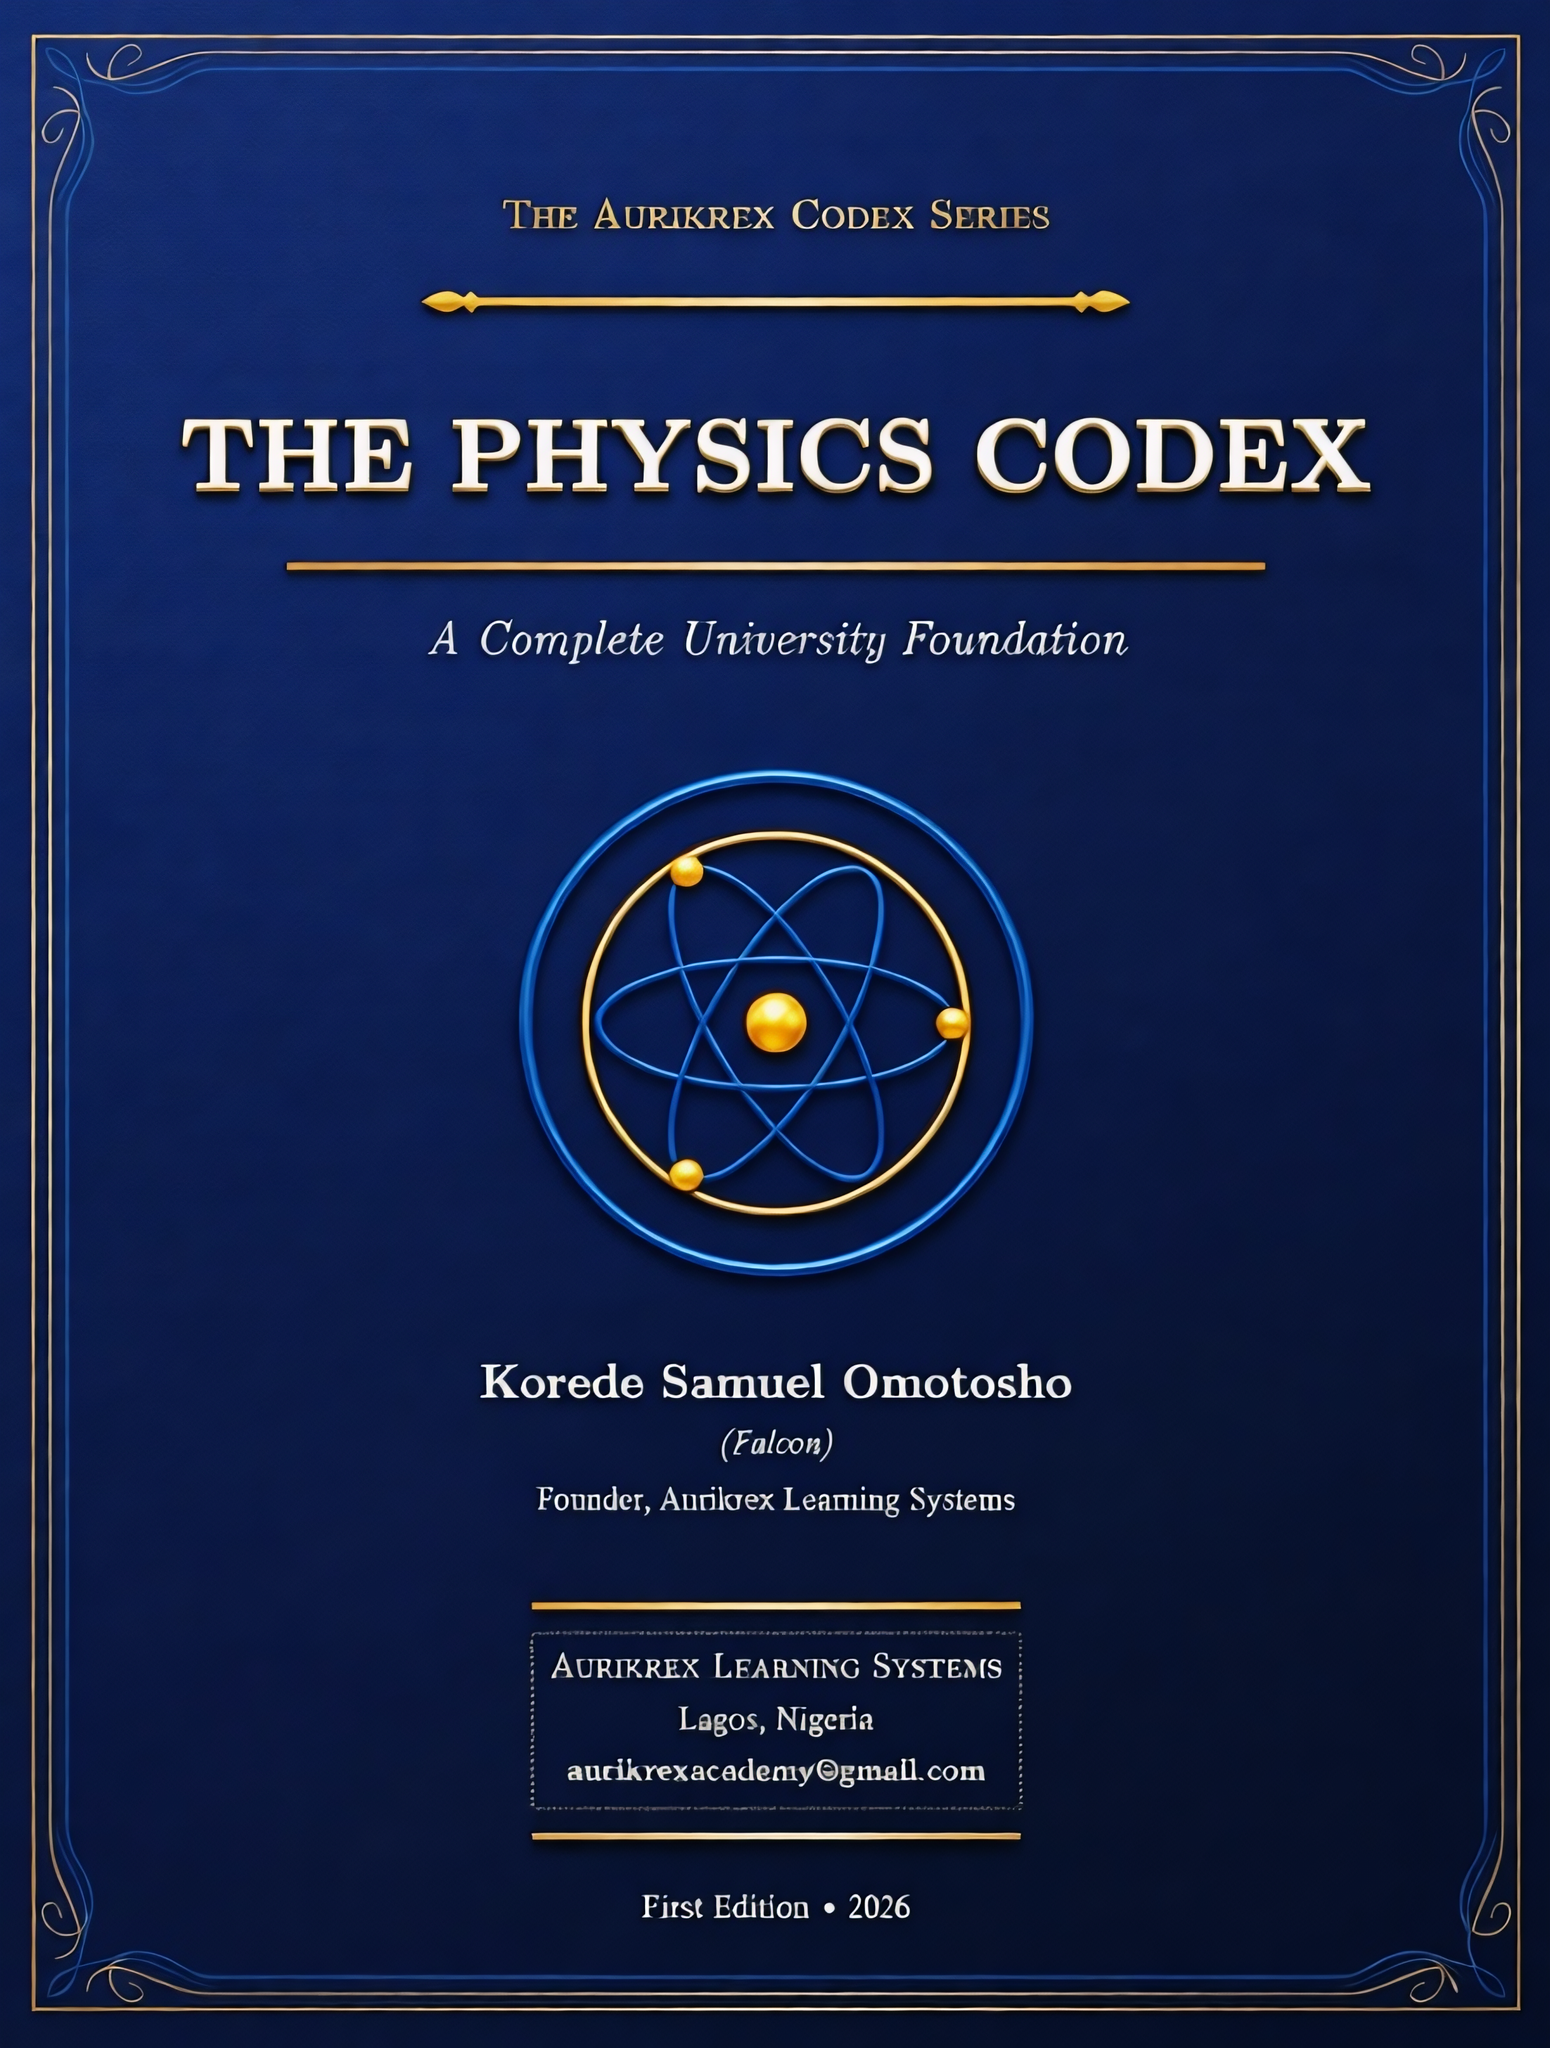
\includegraphics[width=\paperwidth,height=\paperheight,keepaspectratio]{front_cover.png}%
  \end{center}
  \cleardoublepage
}{%
  % (Optional) If you haven't added the cover image yet, compilation still works.
}

% ============================================================
% FRONT MATTER
% ============================================================
\frontmatter
\pagestyle{empty}

\inputifexists{front_matter/titlepage}
\cleardoublepage

\inputifexists{front_matter/copyright}
\cleardoublepage

\inputifexists{front_matter/dedication}
\cleardoublepage

\inputifexists{front_matter/foreword}
\cleardoublepage

\pagestyle{fancy}

\inputifexists{front_matter/preface}
\cleardoublepage

\inputifexists{front_matter/how_to_use}
\cleardoublepage

\inputifexists{front_matter/about_author}
\cleardoublepage

% ============================================================
% TABLE OF CONTENTS
% ============================================================
{
  \hypersetup{linkcolor=black}
  \tableofcontents
}
\cleardoublepage

% List of Figures
\listoffigures
\addcontentsline{toc}{chapter}{List of Figures}
\cleardoublepage

% ============================================================
% MAIN MATTER
% ============================================================
\mainmatter
\pagestyle{fancy}

% ============================================================
% PART 1: MECHANICS
% ============================================================
\part{Mechanics}

\inputifexists{chapters/part1_mechanics/ch01_measurement}
\inputifexists{chapters/part1_mechanics/ch02_scalars_vectors}
\inputifexists{chapters/part1_mechanics/ch03_kinematics}
\inputifexists{chapters/part1_mechanics/ch04_newtons_laws_dynamics}
\inputifexists{chapters/part1_mechanics/ch05_work_energy_power}
\inputifexists{chapters/part1_mechanics/ch06_circular_motion}
\inputifexists{chapters/part1_mechanics/ch07_simple_harmonic_motion}
\inputifexists{chapters/part1_mechanics/ch08_gravitation}

\inputifexists{chapters/part1_mechanics/ch09_elasticity}

\inputifexists{chapters/part1_mechanics/ch10_simple_machines}


% ============================================================
% PART 2: FLUIDS AND THERMAL PHYSICS
% ============================================================
\part{Fluids and Thermal Physics}

\inputifexists{chapters/part2_fluids_thermal/ch11_density_pressure_archimedes}
\inputifexists{chapters/part2_fluids_thermal/ch12_surface_tension_viscosity_capillarity}
\inputifexists{chapters/part2_fluids_thermal/ch13_temperature_thermal_expansion}
\inputifexists{chapters/part2_fluids_thermal/ch14_gas_laws_kinetic_theory}
\inputifexists{chapters/part2_fluids_thermal/ch15_heat_energy_calorimetry}
\inputifexists{chapters/part2_fluids_thermal/ch16_heat_transfer}

% ============================================================
% PART 3: WAVES AND OPTICS
% ============================================================
\part{Waves and Optics}

\inputifexists{chapters/part3_waves_optics/ch17_wave_motion}
\inputifexists{chapters/part3_waves_optics/ch18_sound_waves}
\inputifexists{chapters/part3_waves_optics/ch19_light_reflection}
\inputifexists{chapters/part3_waves_optics/ch20_light_refraction_optical_instruments}

% ============================================================
% PART 4: ELECTRICITY AND MAGNETISM
% ============================================================
\part{Electricity and Magnetism}

\inputifexists{chapters/part4_electricity_magnetism/ch21_electrostatics}
\inputifexists{chapters/part4_electricity_magnetism/ch22_capacitance}
\inputifexists{chapters/part4_electricity_magnetism/ch23_current_electricity}
\inputifexists{chapters/part4_electricity_magnetism/ch24_electrical_energy_power}
\inputifexists{chapters/part4_electricity_magnetism/ch25_magnetism_electromagnetism}
\inputifexists{chapters/part4_electricity_magnetism/ch26_electromagnetic_induction}

% ============================================================
% PART 5: MODERN PHYSICS
% ============================================================
\part{Modern Physics}

\inputifexists{chapters/part5_modern_physics/ch27_atomic_structure_spectra}
\inputifexists{chapters/part5_modern_physics/ch28_radioactivity_nuclear_physics}
\inputifexists{chapters/part5_modern_physics/ch29_electronics}

% ============================================================
% BACK MATTER
% ============================================================
\backmatter
\pagestyle{fancy}

% ============================================================
% APPENDICES
% ============================================================
\appendix
\part*{Appendices}
\addcontentsline{toc}{part}{Appendices}
\inputifexists{back_matter/appendix_a_constants}
\inputifexists{back_matter/appendix_b_formulae}
\inputifexists{back_matter/appendix_c_si_units}


% ============================================================
% ANSWERS TO EXERCISES
% ============================================================
\inputifexists{back_matter/answers}

% ============================================================
% BIBLIOGRAPHY
% ============================================================
\inputifexists{back_matter/bibliography}

% ============================================================
% INDEX
% ============================================================
\printindex

% ============================================================
% BACK COVER
% ============================================================
\IfFileExists{back_cover.png}{%
  \cleardoublepage
  \thispagestyle{empty}%
  \begin{center}
    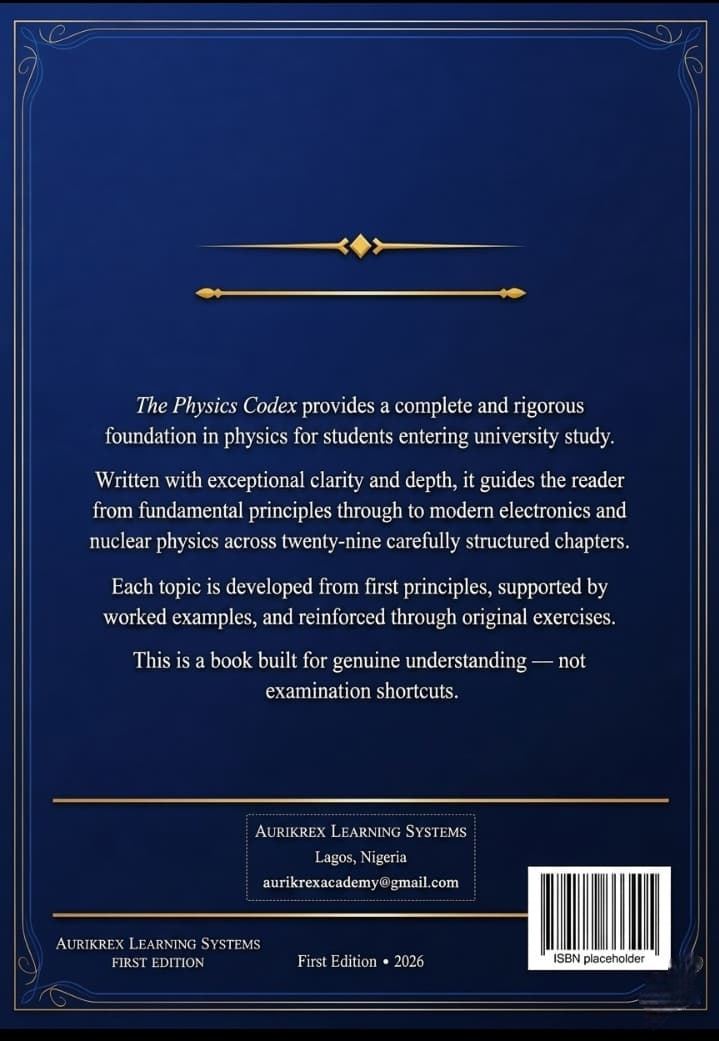
\includegraphics[width=\paperwidth,height=\paperheight,keepaspectratio]{back_cover.png}%
  \end{center}
}{%
  % (Optional) If you haven't added the back cover image yet, compilation still works.
}

\end{document}
